\chapter{МОДЕЛИРОВАНИЕ РОСТА ТРЕЩИН АВТОГРП В ДЛИНУ} \label{ch4}

\section{Постановка задачи}
\vspace*{-5mm}

На основе модели одномерных утечек Картера \cite{karter} в работе \cite{koning} получена первая формула Кёнинга, которая представляет собой зависимость полудлины трещины автоГРП от расхода жидкости, фильтрационно-ёмкостных свойств (ФЕС) пласта, репрессии на пласт и времени:
\beq\label{Koning_first}
x_{\!f}=\frac{Q\mu\sqrt{\pi\kappa t}}{2\pi k_eh\left(p_{\!f}-p_e\right)},
\eeq
где $Q$ -- расход нагнетаемой в рассматриваемую трещину жидкости;
$\mu$ -- вязкость жидкости;
$\kappa=k_e/(\varphi_e\mu c_t)$ -- коэффициент пьезопроводности пласта;
$t$ -- время закачки;
$k_e$ -- проницаемость пласта;
$\varphi_e$ -- пористость пласта;
$c_t$ -- общая сжимаемость системы (состоит из сжимаемости флюидов и сжимаемости порового пространства);
$h$ -- эффективная толщина (мощность) пласта;
$\Delta p=p_{\!f}-p_e$ -- разница между средним давлением в трещине и пластовым давлением (репрессия на пласт).\\

В текущей работе рассматривается одновременный рост нескольких трещин гидроразрыва, поэтому расход жидкости на каждой из них может динамично меняться согласно правилам Кирхгофа.
Кроме того, давление в трещинах в общем случае тоже может меняться по мере увеличения объёма трещин и изменения расхода на них.
Получается, что согласно формуле \eqref{Koning_first} есть зависимость полудлины трещины $x_{\!f}$ от расхода на трещине $Q$, но при этом на расход в общем случае может влиять текущая полудлина каждой из трещин.

Таким образом, для корректного применения формулы Кёнинга приращение полудлины каждой из трещин на текущем шаге по времени необходимо найти как произведение полной производной формулы Кёнинга по времени и рассматриваемого временного шага.\newline
Полная производная полудлины трещины $x_{\!f}$ по времени $t$:
\beq\label{FullDerivative}
\frac{dx_{\!f}}{dt}=\frac{\partial x_{\!f}}{\partial t}+\frac{\partial x_{\!f}}{\partial Q}\frac{dQ}{dt}+\frac{\partial x_{\!f}}{\partial (p_{\!f}-p_e)}\frac{d(p_{\!f}-p_e)}{dt}
\eeq
Частная производная полудлины трещины $x_{\!f}$ по времени $t$:
\beq\label{PartialDerivative_t_first}
\frac{\partial x_{\!f}}{\partial t}=\frac{Q\mu}{4\pi k_eh\left(p_{\!f}-p_e\right)}\sqrt{\frac{\pi\kappa}{t}}
\eeq
Частная производная полудлины трещины $x_{\!f}$ по расходу $Q$:
\beq\label{PartialDerivative_Q_first}
\frac{\partial x_{\!f}}{\partial Q}=\frac{\mu\sqrt{\pi\kappa t}}{2\pi k_eh\left(p_{\!f}-p_e\right)}
\eeq
Частная производная полудлины трещины $x_{\!f}$ по репрессии на пласт $\left(p_{\!f}-p_e\right)$:
\beq\label{PartialDerivative_p_first}
\frac{\partial x_{\!f}}{\partial (p_{\!f}-p_e)}=-\frac{Q\mu\sqrt{\pi\kappa t}}{2\pi k_eh\left(p_{\!f}-p_e\right)^2}
\eeq
Подставляя \eqref{PartialDerivative_t_first}, \eqref{PartialDerivative_Q_first} и \eqref{PartialDerivative_p_first} в выражение \eqref{FullDerivative}, получаем:
\beq\label{FullDerivativeExplicit_first}
\frac{dx_{\!f}}{dt}=\frac{\mu}{2\pi k_e h(p_{\!f}-p_e)}\left(\frac{Q}{2}\sqrt{\frac{\pi\kappa}{t}}+\sqrt{\pi\kappa t}\,\frac{dQ}{dt}-\frac{Q\sqrt{\pi\kappa t}}{\left(p_{\!f}-p_e\right)}\frac{d(p_{\!f}-p_e)}{dt}\right)
\eeq
             
Итак, приращение полудлины трещины на каждом шаге по времени при рассмотрении случая одномерных утечек Картера записывается в следующем виде:
\beq\label{IncrementExplicit_first}
dx_{\!f}=\frac{\mu}{2\pi k_e h(p_{\!f}-p_e)}\left(\frac{Q}{2}\sqrt{\frac{\pi\kappa}{t}}dt+\sqrt{\pi\kappa t}\,dQ-\frac{Q\sqrt{\pi\kappa t}}{\left(p_{\!f}-p_e\right)}d(p_{\!f}-p_e)\right)
\eeq\\

Дополнительно в работе \cite{koning} получена вторая формула Кёнинга, которая применяется в случае двумерных радиальных утечек жидкости из трещины в пласт и представляет собой зависимость полудлины трещины автоГРП от расхода жидкости, фильтрационно-ёмкостных свойств (ФЕС) пласта, репрессии на пласт и времени:
\beq\label{Koning_second}
x_{\!f}=3\exp{\!\left(-\frac{2\pi k_e h\left(p_{\!f}-p_e\right)}{Q\mu}\right)}\sqrt{\kappa t}
\eeq
В этом случае частная производная полудлины трещины $x_{\!f}$ по времени $t$:
\beq\label{PartialDerivative_t_second}
\frac{\partial x_{\!f}}{\partial t}=\frac{3}{2}\exp{\left(-\frac{2\pi k_e h \left(p_{\!f}-p_e\right)}{Q\mu}\right)}\sqrt{\frac{\kappa}{t}}
\eeq
Частная производная полудлины трещины $x_{\!f}$ по расходу $Q$:
\beq\label{PartialDerivative_Q_second}
\frac{\partial x_{\!f}}{\partial Q}=\frac{6\pi k_e h\left(p_{\!f}-p_e\right)}{Q^2\mu}\exp{\!\left(-\frac{2\pi k_e h\left(p_{\!f}-p_e\right)}{Q\mu}\right)}\sqrt{\kappa t}
\eeq
Частная производная полудлины трещины $x_{\!f}$ по репрессии на пласт $\left(p_{\!f}-p_e\right)$:
\beq\label{PartialDerivative_p_second}
\frac{\partial x_f}{\partial (p_{\!f}-p_e)}=-\frac{6\pi k_e h}{Q\mu}\exp{\!\left(-\frac{2\pi k_e h\left(p_{\!f}-p_e\right)}{Q\mu}\right)}\sqrt{\kappa t}
\eeq

Подставляя \eqref{PartialDerivative_t_second}, \eqref{PartialDerivative_Q_second} и \eqref{PartialDerivative_p_second} в выражение \eqref{FullDerivative}, получаем:
\beq
\begin{gathered}
\frac{dx_{\!f}}{dt}=\exp{\!\left(-\frac{2\pi k_e h\left(p_{\!f}-p_e\right)}{Q\mu}\right)}\left(\frac{3}{2}\sqrt{\frac{\kappa}{t}}\,+\right.\\[10pt]
+\left.\frac{6\pi k_e h\left(p_{\!f}-p_e\right)}{Q^2\mu}\sqrt{\kappa t}\,\frac{dQ}{dt}-\frac{6\pi k_e h}{Q\mu}\sqrt{\kappa t}\,\frac{d(p_{\!f}-p_e)}{dt}\right)
\end{gathered}
\eeq

Итак, приращение полудлины трещины на каждом шаге по времени при рассмотрении случая двумерных радиальных утечек жидкости из трещины в пласт записывается в следующем виде:
\beq\label{IncrementExplicit_second}
\begin{gathered}
dx_{\!f}=\exp{\!\left(-\frac{2\pi k_e h\left(p_{\!f}-p_e\right)}{Q\mu}\right)}\left(\frac{3}{2}\sqrt{\frac{\kappa}{t}}dt\,+\right.\\[10pt]
+\left.\frac{6\pi k_e h\left(p_{\!f}-p_e\right)}{Q^2\mu}\sqrt{\kappa t}\,dQ-\frac{6\pi k_e h}{Q\mu}\sqrt{\kappa t}\,d(p_{\!f}-p_e)\right)
\end{gathered}
\eeq

Постановка задачи принимает следующий вид: используя решатель уравнений Кирхгофа, реализованный в главе \ref{ch3}, и формулы для приращения полудлины трещины \eqref{IncrementExplicit_first} и \eqref{IncrementExplicit_second}, построить графики зависимостей полудлины трещины и расхода на трещинах от времени при одномерных утечках Картера и при двумерных радиальных утечках жидкости из трещины в пласт.

\section{Описание численного алгоритма решения}
\vspace*{-5mm}

Совмещение формулы Кёнинга с уравнениями Кирхгофа проводится следующим образом:

1) на текущем шаге по времени по имеющимся значениям полудлины трещин автоГРП предыдущего шага рассчитываются давления и расходы на каждой трещине;

2) на основе полученных значений приращений давления и расхода рассчитывается приращение полудлины трещины $dx_{\!f}$ на данном временном шаге по формуле \eqref{IncrementExplicit_first} в случае одномерных утечек Картера и по формуле \eqref{IncrementExplicit_second} в случае двумерных радиальных утечек жидкости из трещины в пласт;

3) по формуле $x_{\!f}^{\text{current}}=x_{\!f}^{\text{last}}+dx_{\!f}$ рассчитываются полудлины каждой из трещин на текущем временном шаге;

4) описанные действия повторяются до требуемого шага по времени (условия остановки).

На рис. \ref{fig:koning_scheme} этот алгоритм расчёта полудлин растущих трещин автоГРП представлен в виде блок-схемы.

\begin{figure}[H] 
\center
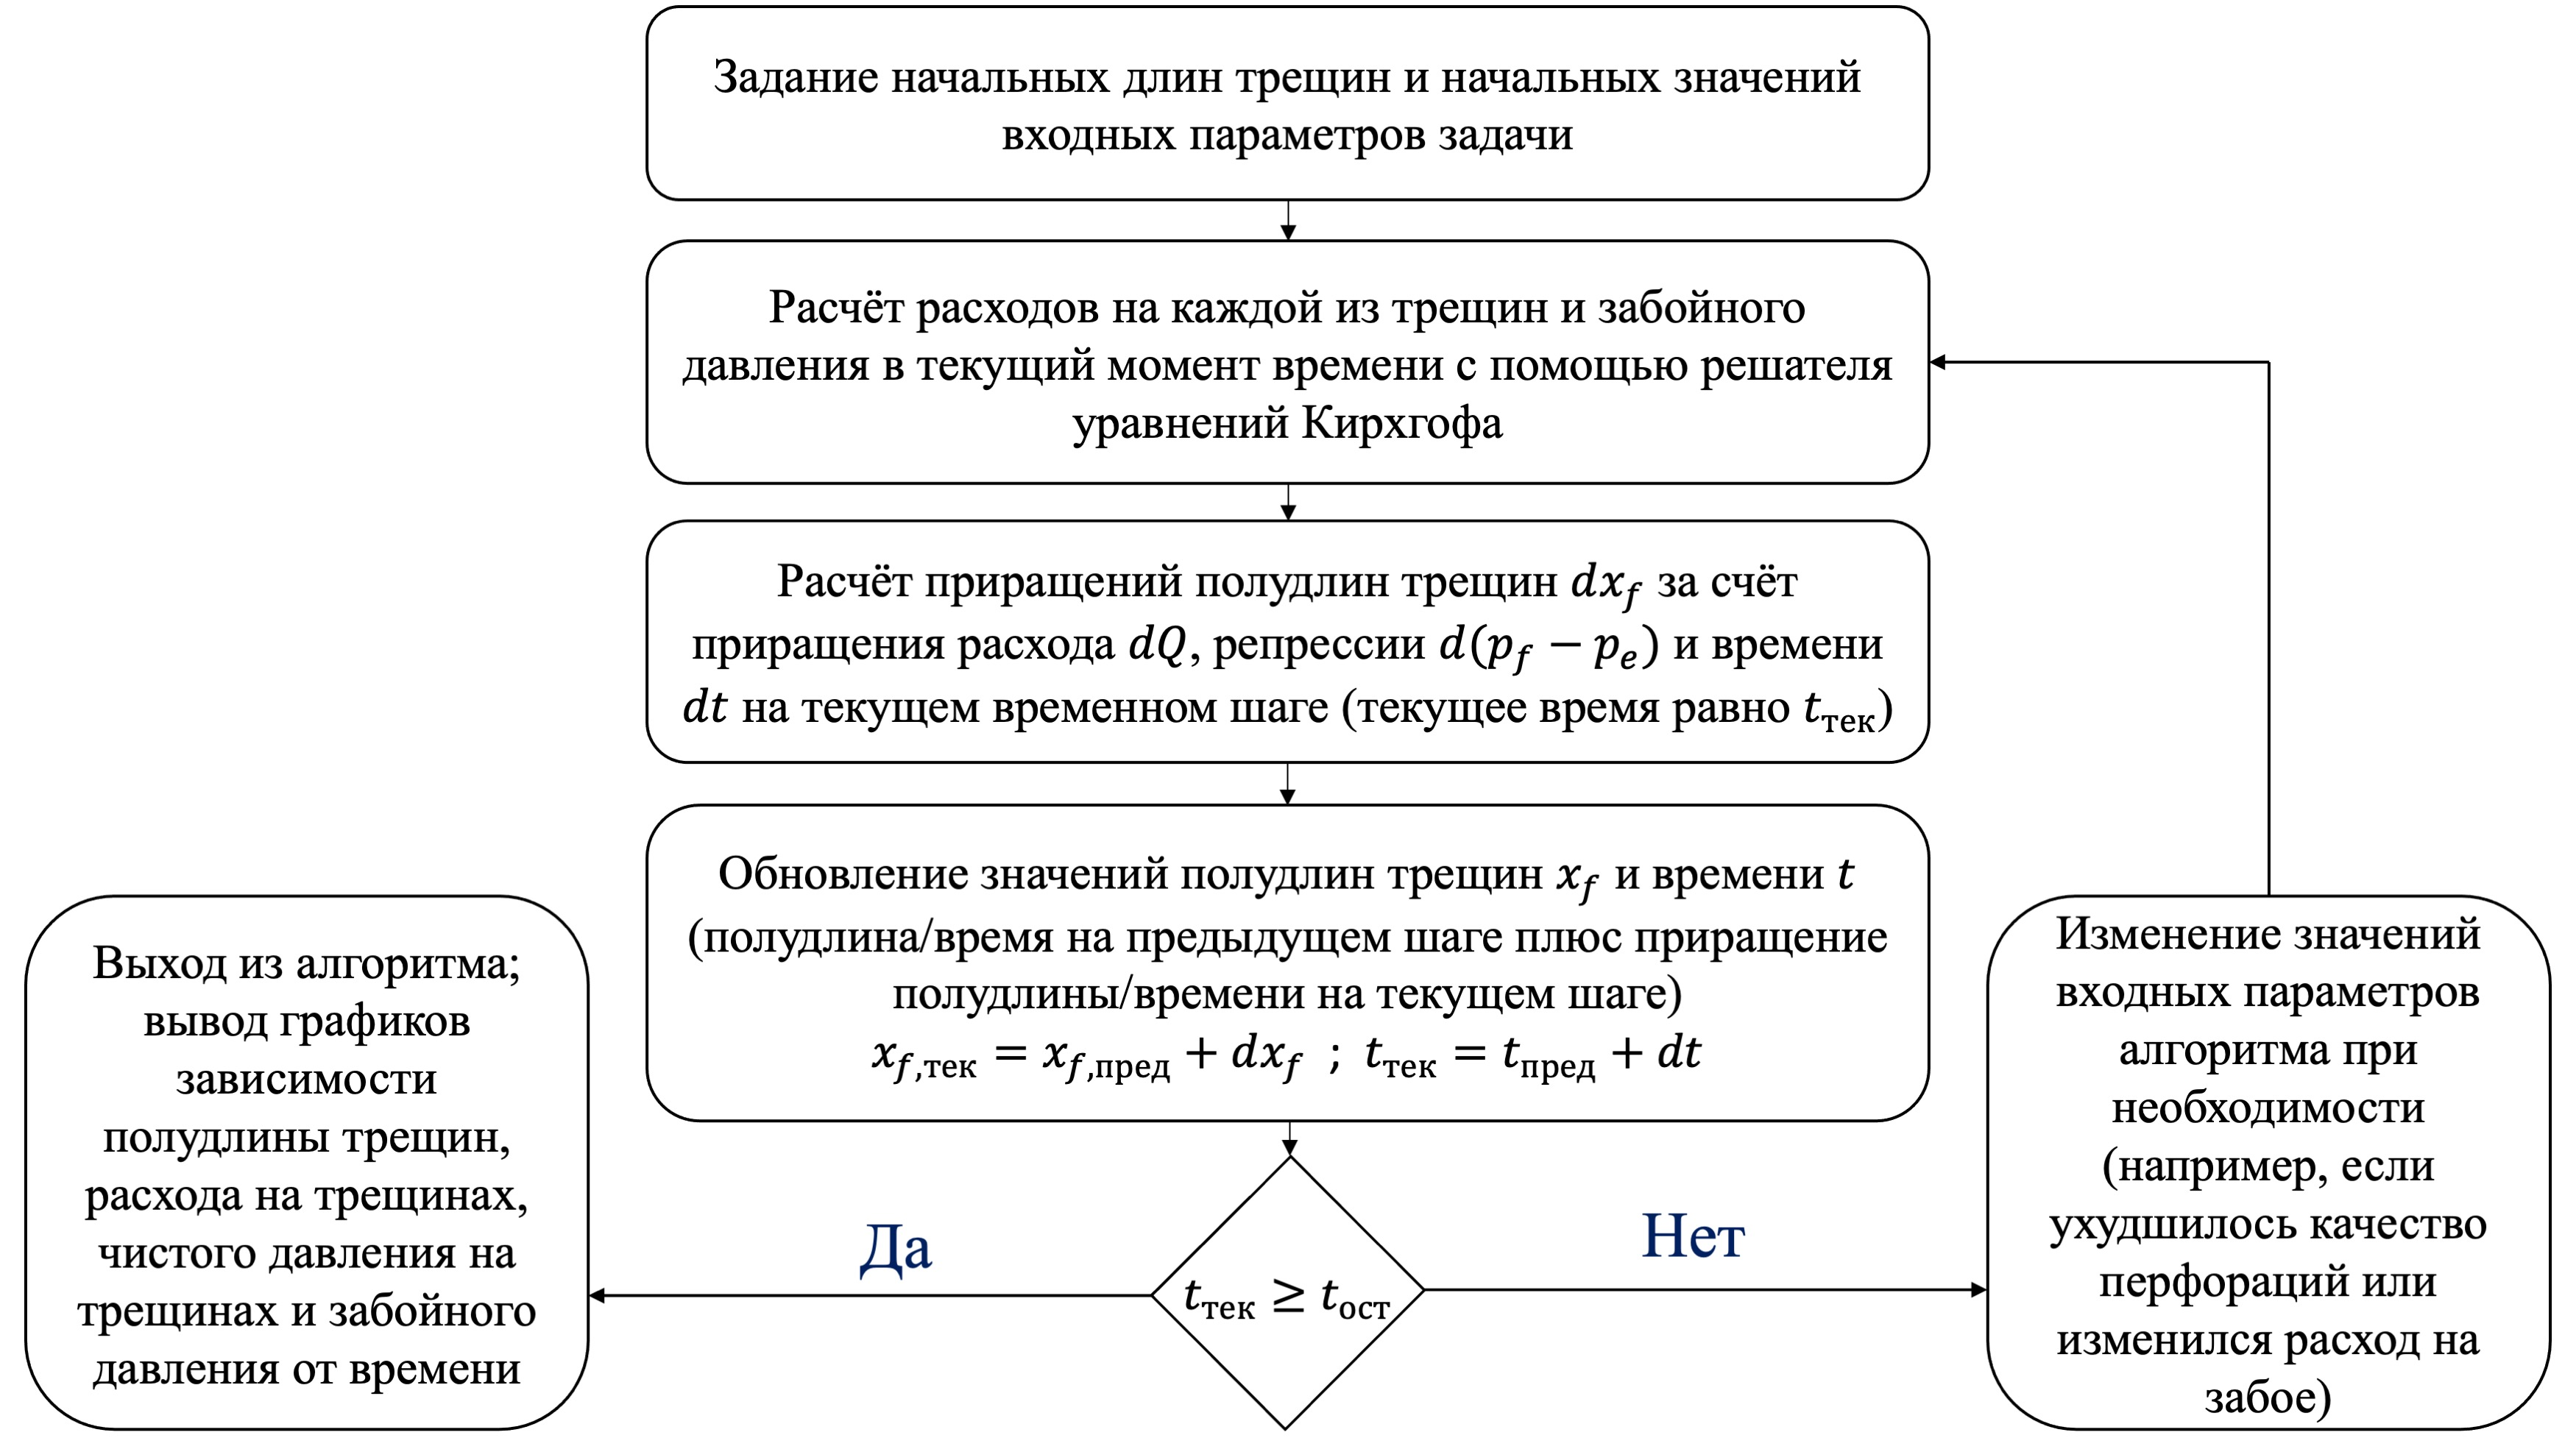
\includegraphics[width=\linewidth]{images/Koning_scheme.jpg}
\caption{Алгоритм расчёта полудлин трещин в зависимости от времени} 
\label{fig:koning_scheme}
\end{figure}

Реализация описанного алгоритма решения на языке программирования Python представлена в приложении \ref{appendix-fractures-growth-modelling}.

\section{Результаты моделирования}
\vspace*{-5mm}

Значения входных параметров, выбранные перед запуском алгоритма представлены в таблице \ref{tab:input-parameters-for-fractures-growth}.

\newcolumntype{L}[1]{>{\raggedright\arraybackslash}m{#1}}
\newcolumntype{C}[1]{>{\centering\arraybackslash}p{#1}}
\noindent % for correct centering
\begingroup
\small %выставляем шрифт в 12bp
\begin{longtable}[l]{|C{8cm}|C{8cm}|}
	\caption{Значения входных параметров алгоритма расчёта полудлины трещин}%
	\label{tab:input-parameters-for-fractures-growth}% label всегда желательно идти после caption
	\\
	\hline
	\multicolumn{1}{|c|}{\textbf{Параметр}}&\multicolumn{1}{|c|}{\textbf{Значение}}\\ \hline
	\endfirsthead%
	\captionsetup{format=tablenocaption,labelformat=continued} % до caption!
	\caption[]{}\\ % печать слов о продолжении таблицы
	\hline
	\multicolumn{1}{|c|}{\textbf{Параметр}}&\multicolumn{1}{|c|}{\textbf{Значение}}\\ \hline
	\endhead
	\hline
	\endfoot
	\hline
	\endlastfoot
	Расход на забое $Q_0$&1000 м$^3$/сут\\ \hline
	Вязкость закачиваемой жидкости (воды) $\mu$ & $10^{-3}$ Па$\cdot$с\\ \hline
	Плотность закачиваемой жидкости (воды) $\rho$ & 1000 кг/м$^3$\\ \hline
	Проницаемость пласта $k_e$ & 1 мД\\ \hline
	Пористость пласта $\varphi_e$ & 0.2\\ \hline
	Общая сжимаемость $c_t$ & $2.2\cdot 10^{-9}$ Па$^{-1}$\\ \hline
	Пластовое давление $p_e$ & 25 МПа\\ \hline
	Модуль плоской деформации породы $E'$ & $10^4$ МПа\\ \hline
	Мощность (высота) пласта $H$ & 15 м\\ \hline
	Количество перфораций $n_p$ & 32\\ \hline
	Диаметр перфораций $d_p$ & 0.02 м\\ \hline
	Безразмерный коэффициент эрозии $C_d$ & 0.5\\ \hline
	Радиус участков трубы $R$ & 0.08 м\\ \hline
	Длина участков трубы $L$ & 100 м\\ \hline
	Давление смыкания $\sigma_{\text{min}}=\sigma_0$ & 40 МПа\\ \hline
	Трещиностойкость породы $K_{Ic}$ & $10^6$ Па$\cdot$м$^{1/2}$\\ \hline
	Количество трещин & 4\\ \hline
\end{longtable}
\normalsize% возвращаем шрифт к нормальному
\endgroup

На рис. \ref{fig:myimage1} представлены результаты моделирования роста трещин автоГРП при выбранных значениях параметров (см. табл. \ref{tab:input-parameters-for-fractures-growth}) в случае одномерных утечек Картера.

\begin{figure}[H] 
\center
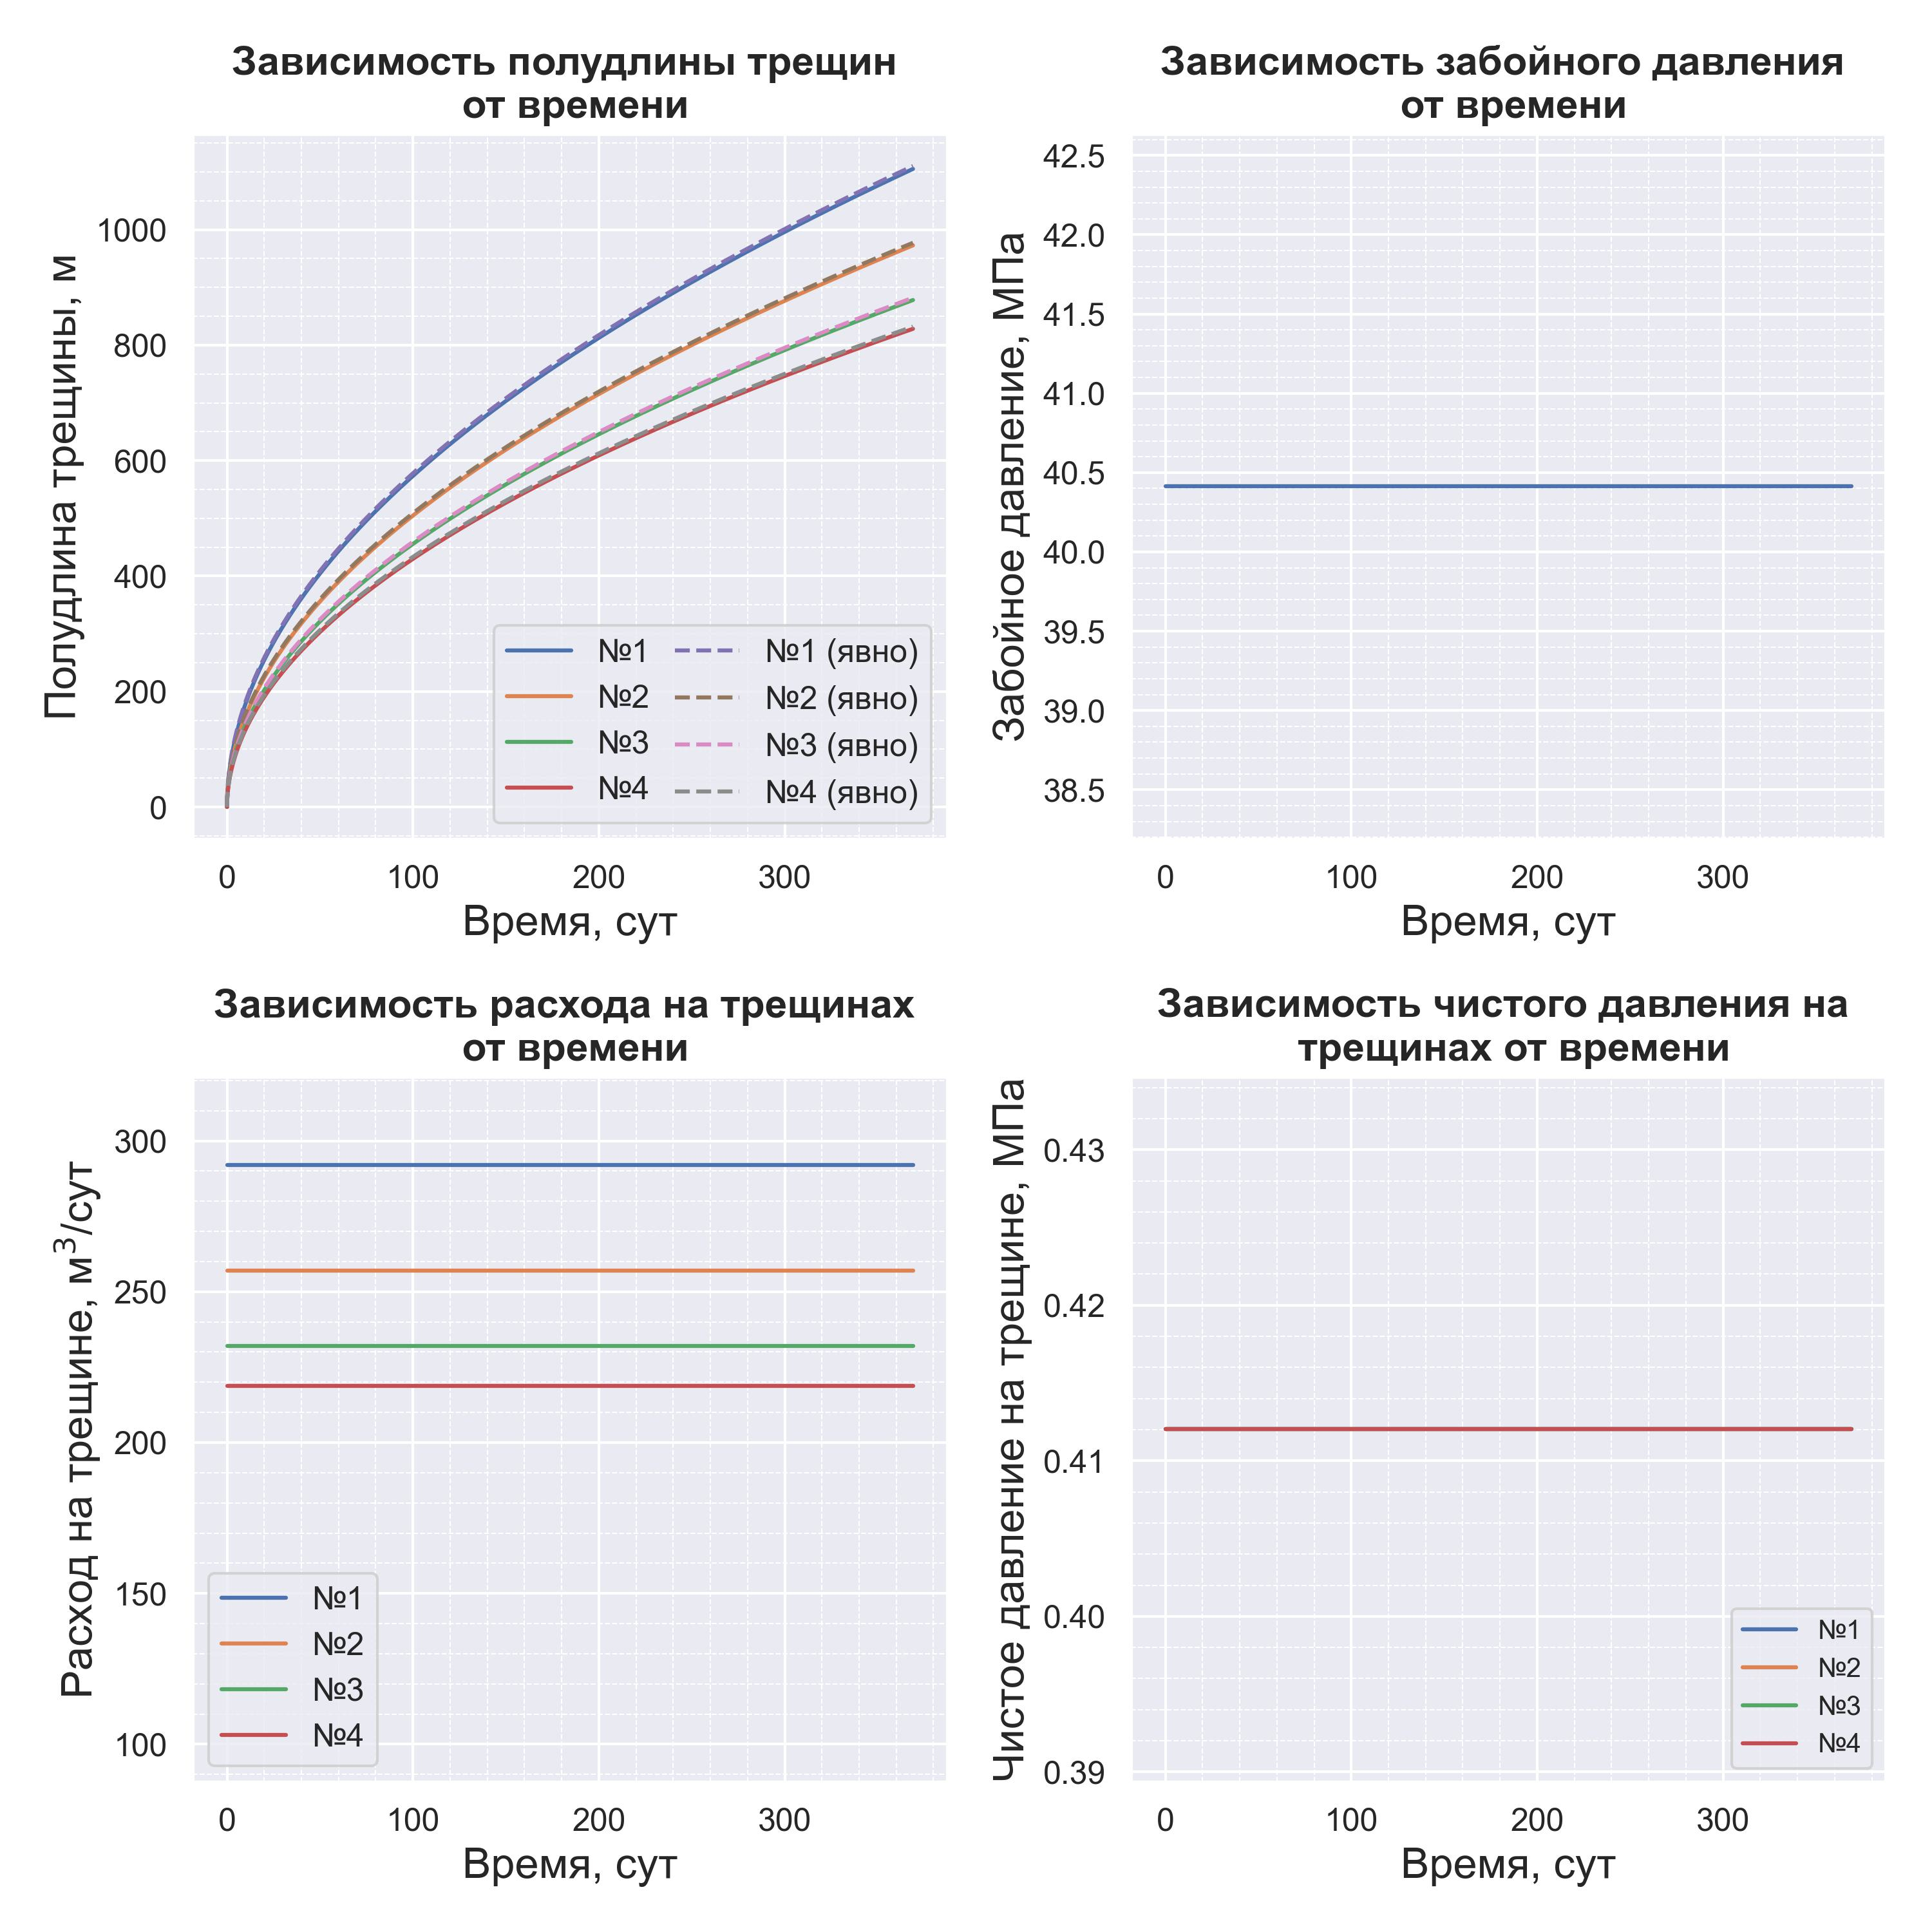
\includegraphics[width=\linewidth]{images/myimage1.jpg}
\caption{Результаты моделирования перераспределения потоков и роста трещин автоГРП в случае одномерных утечек Картера при выбранных значениях входных параметров}
\label{fig:myimage1}
\end{figure}

Видим, что расходы на трещинах постоянны и длина трещин растёт согласно первой формуле Кёнинга \eqref{Koning_first}.
Чистое давление в трещинах постоянно, так как предполагается, что все трещины распространяются и давление в них равно давлению распространения трещин PKN \eqref{p_net_Shel}.
Забойное давление также постоянно, так как расходы (и соответственно перепады давления на трение в трубе и на перфорациях) не меняются со временем.

Такой же эксперимент при выбранных значениях параметров (см. табл. \ref{tab:input-parameters-for-fractures-growth}) проведён в случае двумерных радиальных утечек жидкости из трещины в пласт.
Результаты представлены на рис. \ref{fig:myimage2}.

\begin{figure}[H] 
\center
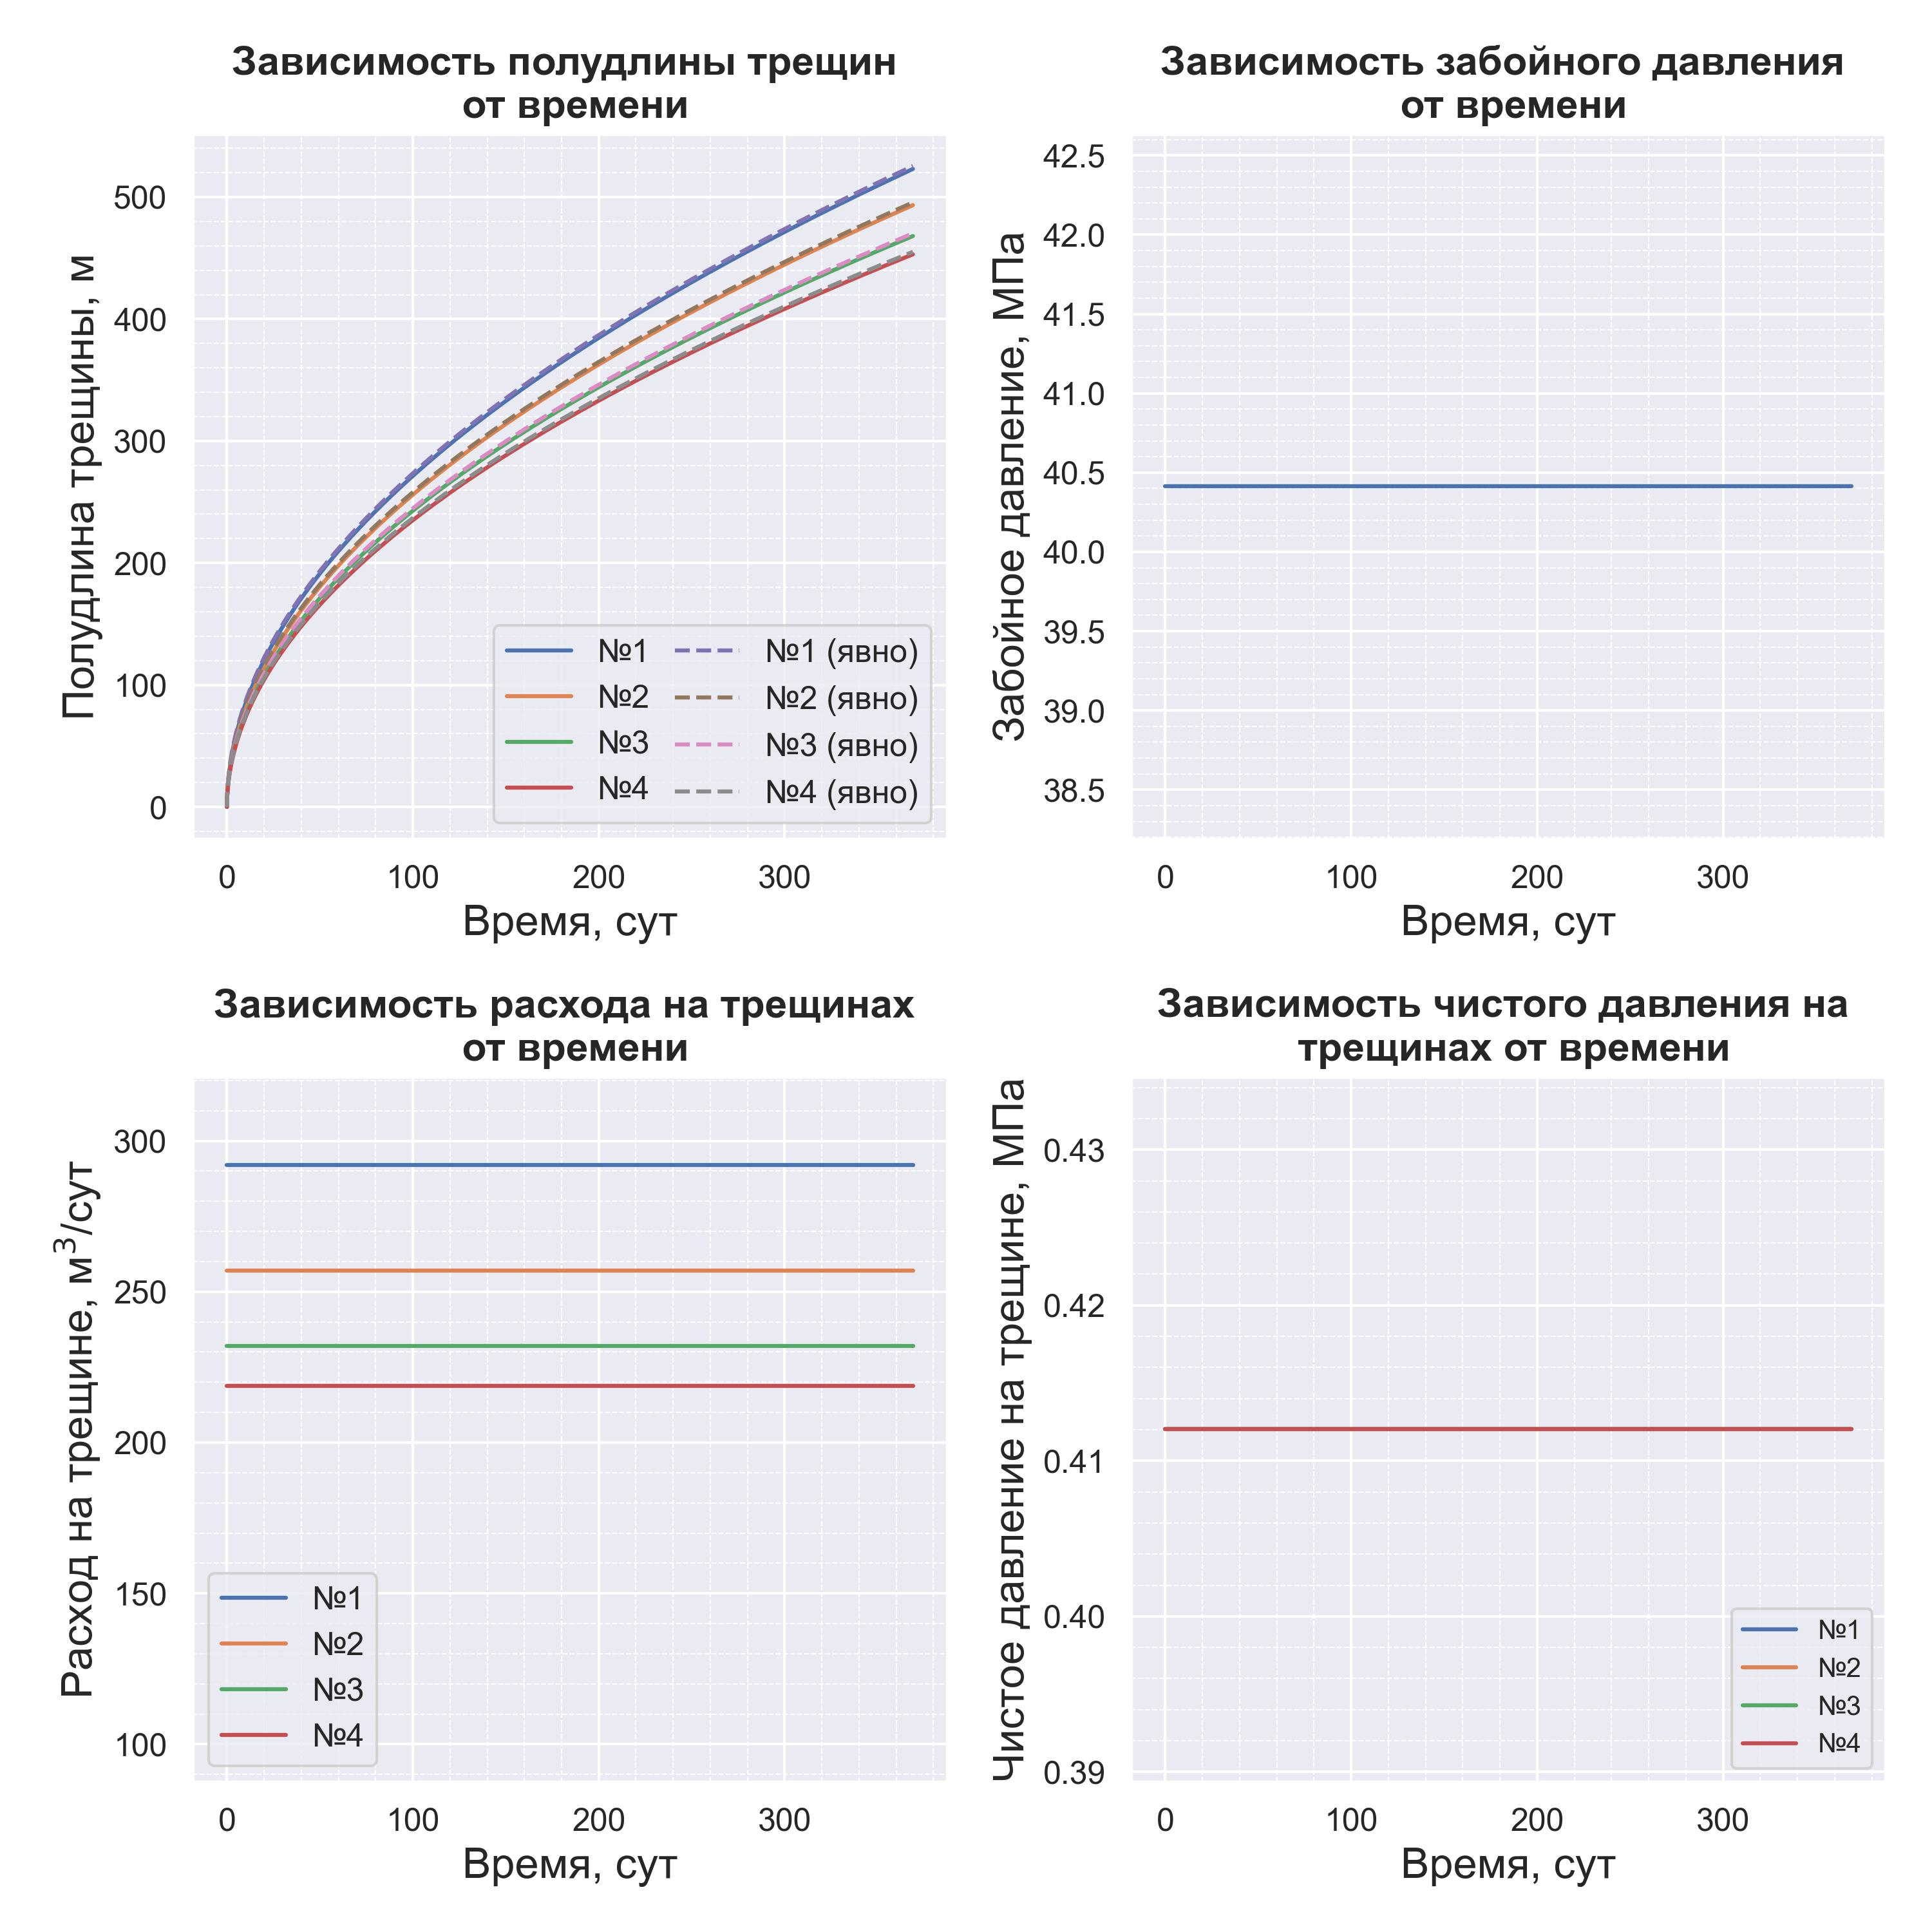
\includegraphics[width=.95\linewidth]{images/myimage2.jpg}
\caption{Результаты моделирования перераспределения потоков и роста трещин автоГРП в случае двумерных радиальных утечек жидкости из трещины при выбранных значениях входных параметров} 
\label{fig:myimage2}
\end{figure}

В этом случае (см. рис. \ref{fig:myimage2}) трещины растут по второй формуле Кёнинга \eqref{Koning_second} и их длина в каждый момент времени меньше, чем длина, полученная в случае одномерных утечек Картера, что согласуется с результатами работы \cite{hagoort}.

Таким образом, предположение одномерности утечек по Картеру \cite{karter} может завышать оценку для длины растущих трещин автоГРП.

На рис. \ref{fig:myimage3} и рис. \ref{fig:myimage4} представлены результаты численного эксперимента при периодическом изменении расхода жидкости на забое скважины по следующей формуле:
\vspace*{-5mm}
\beq
Q_0(t)=1000\frac{\text{м}^3}{\text{сут}}+200\frac{\text{м}^3}{\text{сут}}\cdot\sin{\!\left(\frac{t}{15\text{ сут}}\right)}
\eeq

\begin{figure}[H] 
\center
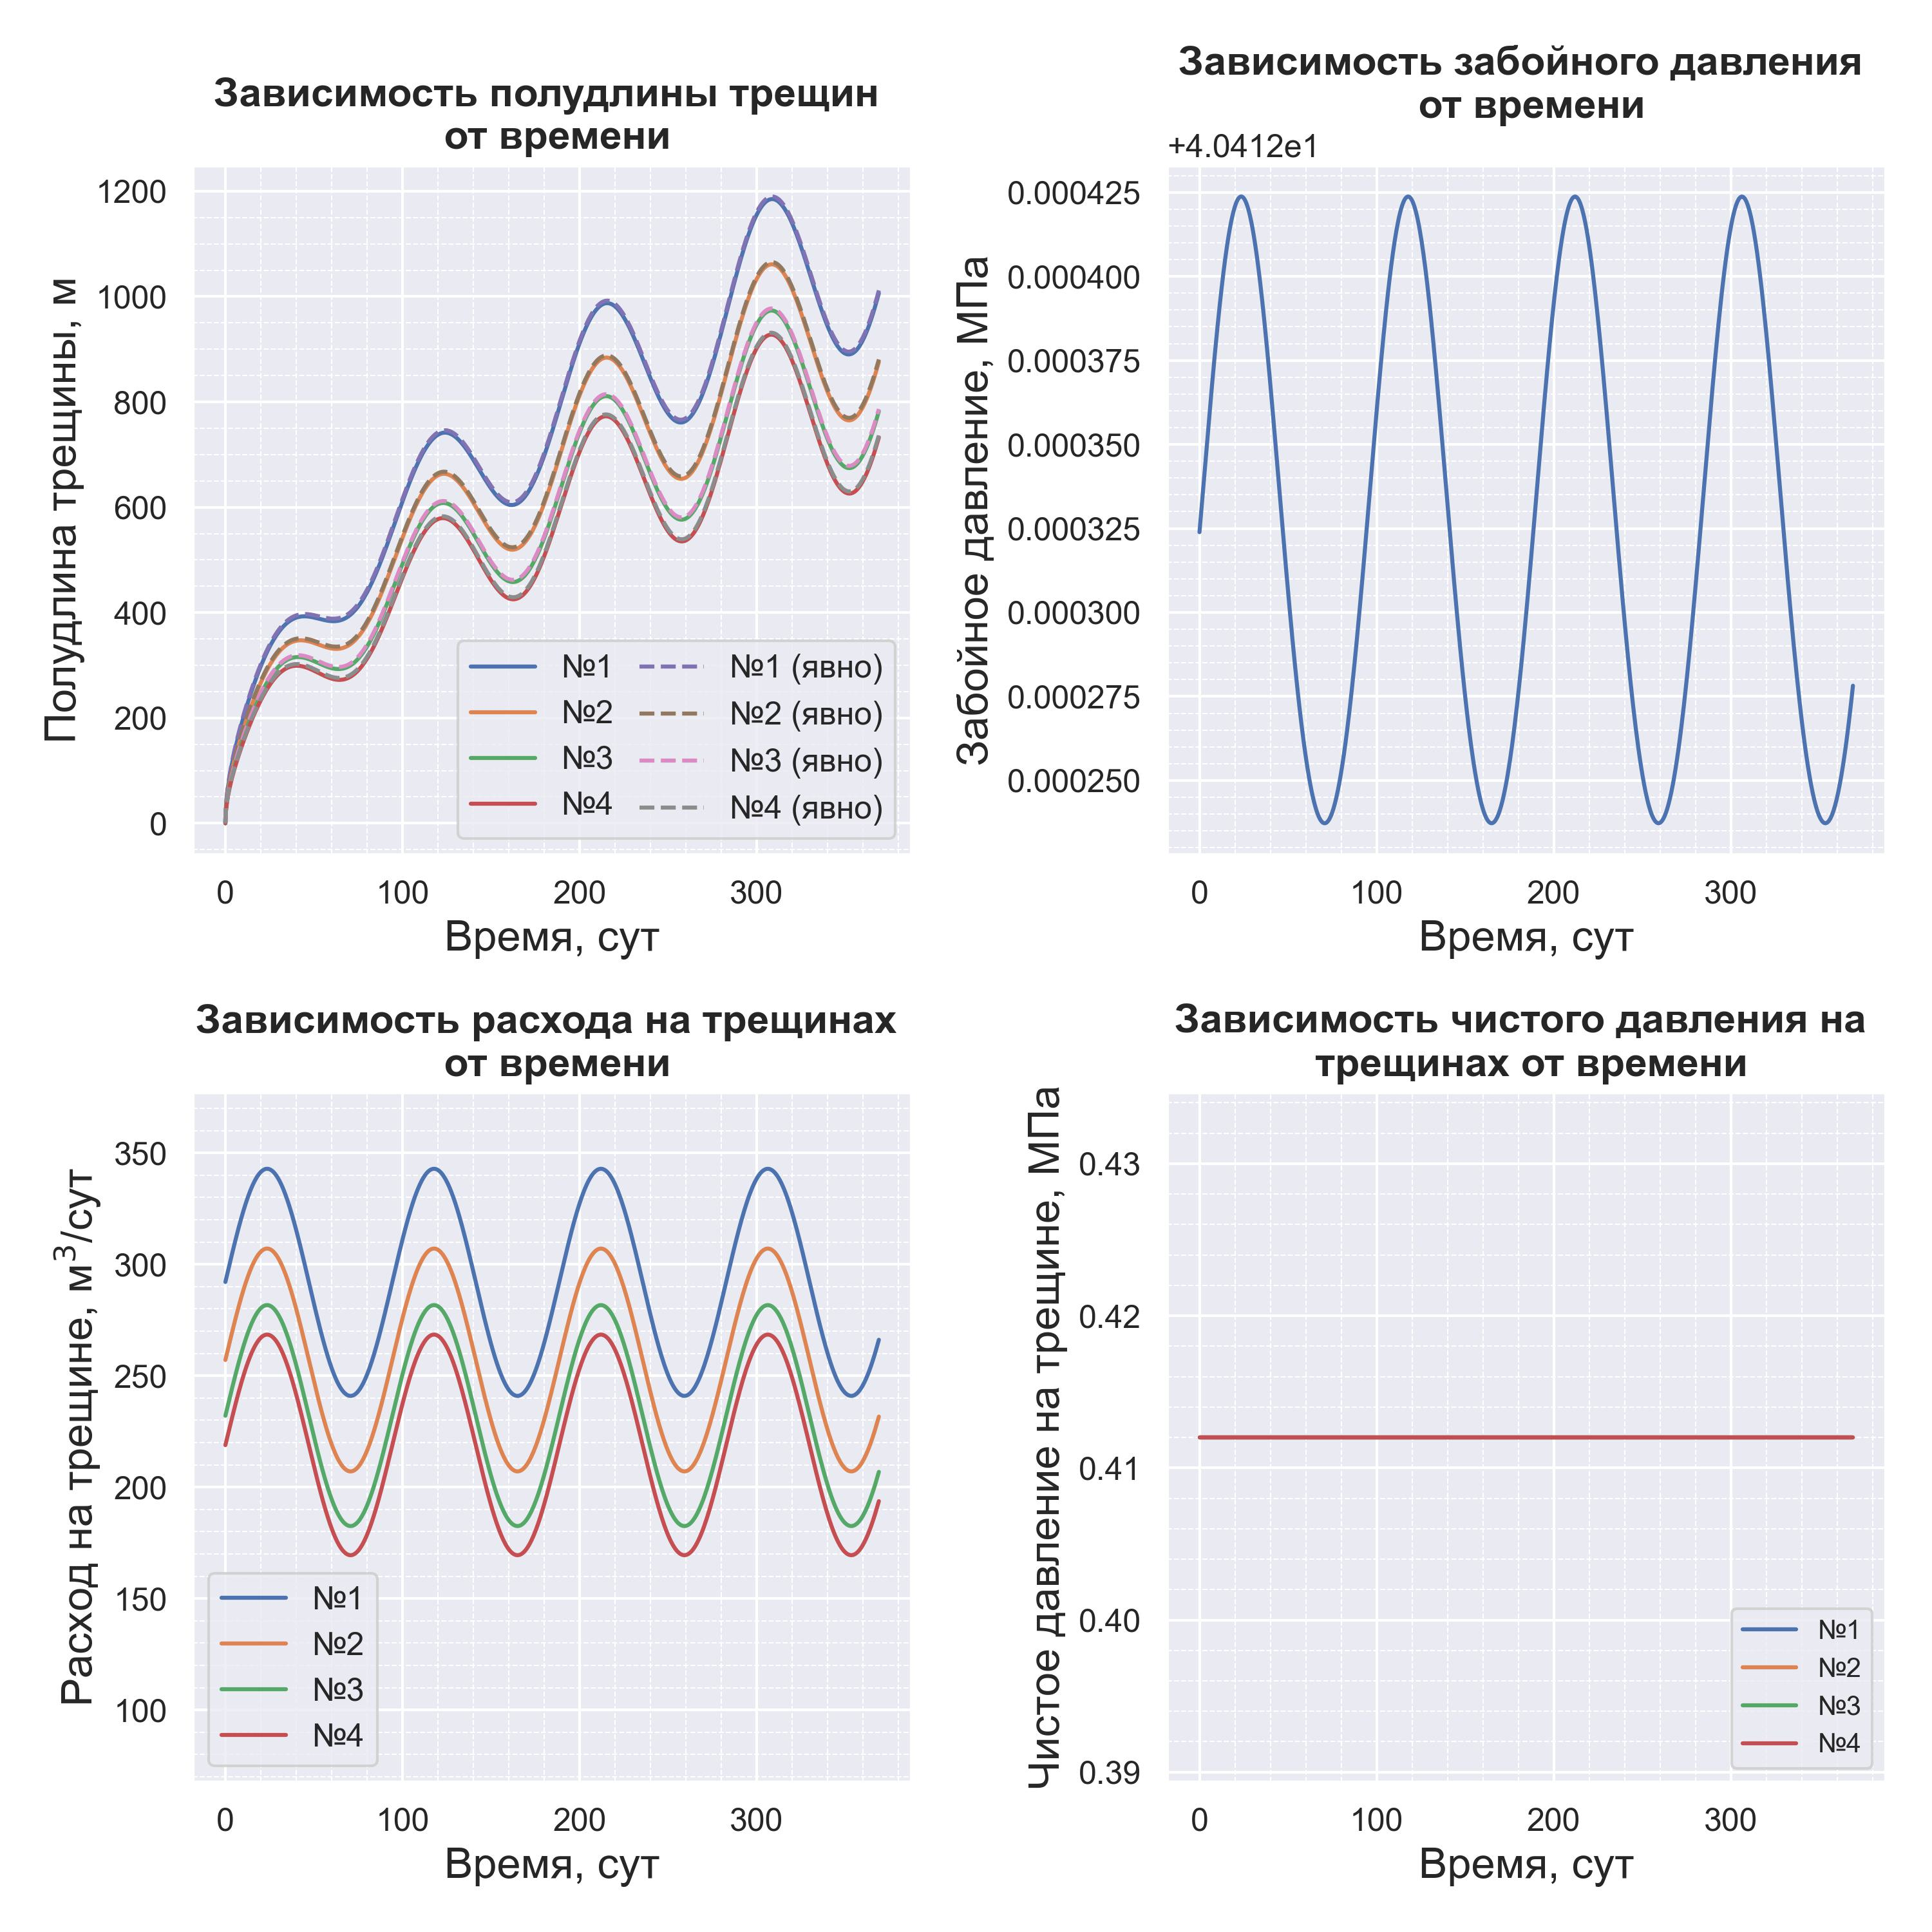
\includegraphics[width=\linewidth]{images/myimage3.jpg}
\caption{Результаты моделирования перераспределения потоков и роста трещин автоГРП в случае 1D утечек Картера и периодическом изменении расхода жидкости на забое скважины} 
\label{fig:myimage3}
\end{figure}

Видим, что при периодическом изменении расхода жидкости на забое скважины, трещины могут как расти, так и уменьшаться в зависимости от конкретного текущего значения расхода, закачиваемого в скважину (см. рис. \ref{fig:myimage3} и \ref{fig:myimage4}).
Но так как значение расхода на забое в среднем остаётся равным $1000\text{ м}^3/\text{сут}$, то общий тренд зависимостей полудлины трещин от времени растущий.

\begin{figure}[H] 
\center
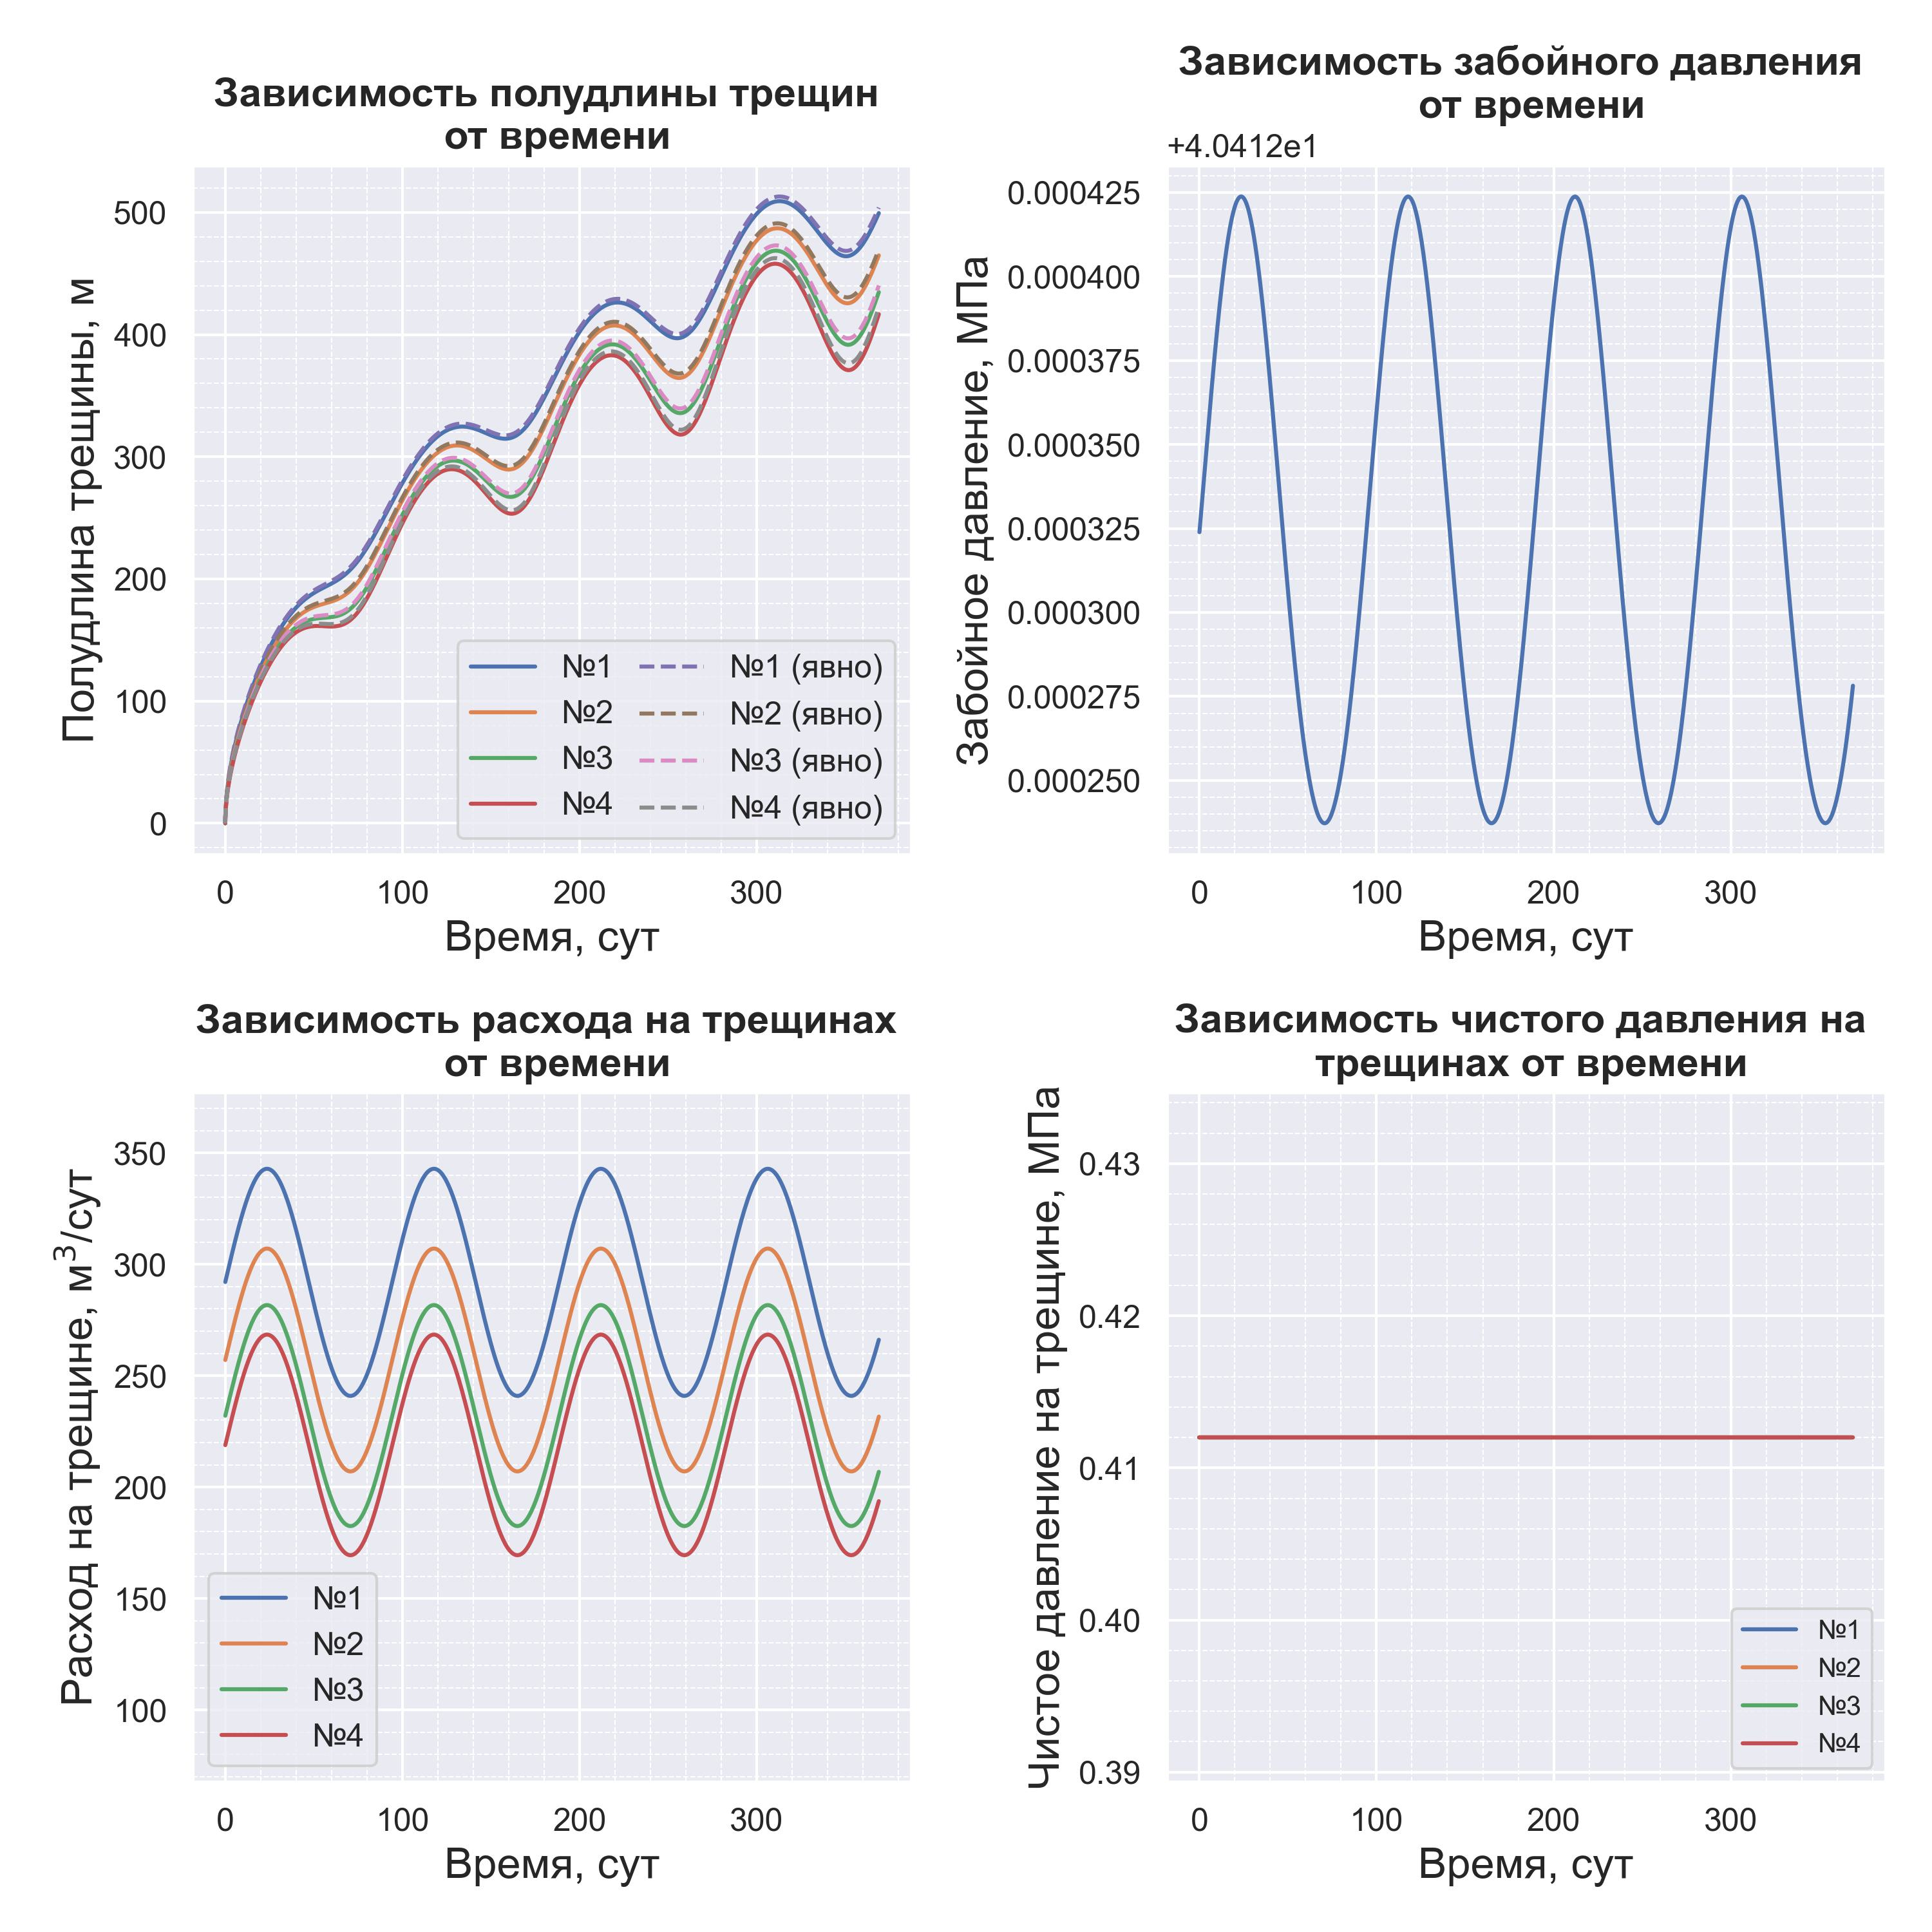
\includegraphics[width=\linewidth]{images/myimage4.jpg}
\caption{Результаты моделирования перераспределения потоков и роста трещин автоГРП в случае двумерных радиальных утечек жидкости из трещины в пласт и периодическом изменении расхода жидкости на забое скважины}
\label{fig:myimage4}
\end{figure}

Далее на рис. \ref{fig:myimage5} и рис. \ref{fig:myimage6} представлены результаты моделирования в случае линейного уменьшения расхода жидкости на забое скважины по следующей формуле:
\beq
Q_0(t)=1200\frac{\text{м}^3}{\text{сут}}-600\frac{\text{м}^3}{\text{сут}}\cdot\left(\frac{t}{365\text{ сут}}\right)
\eeq

\begin{figure}[H] 
\center
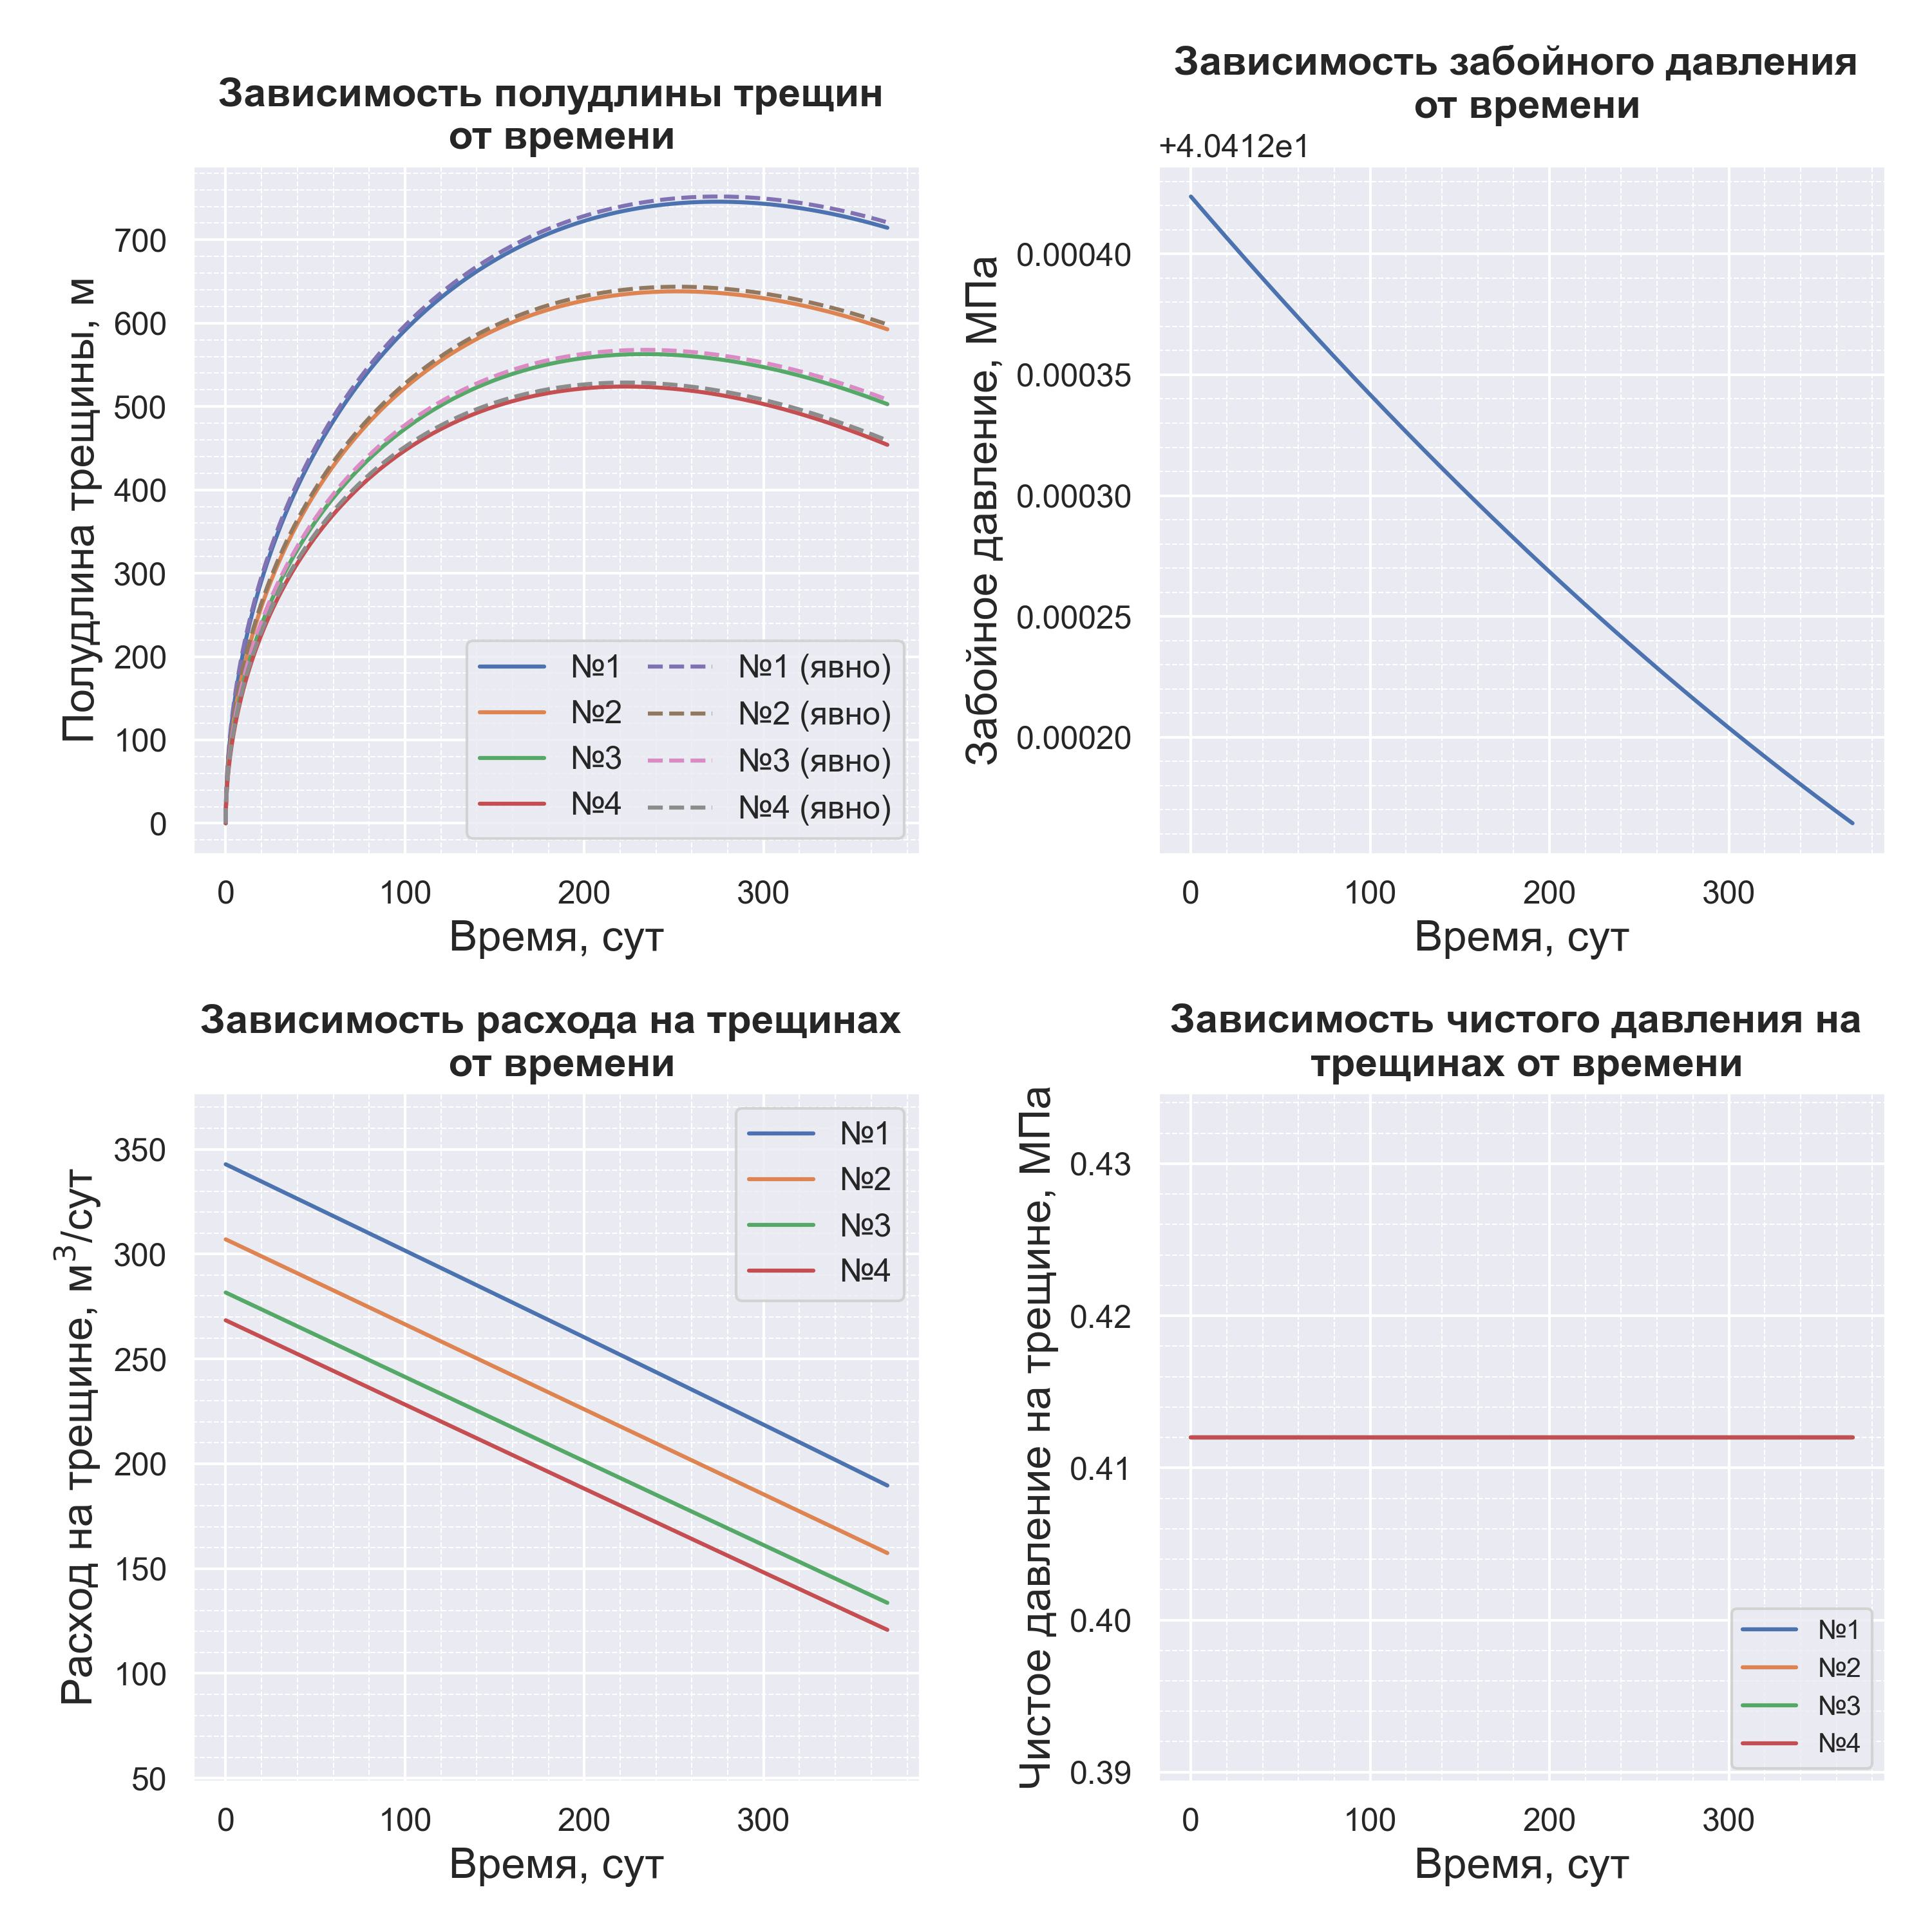
\includegraphics[width=\linewidth]{images/myimage5.jpg}
\caption{Результаты моделирования перераспределения потоков и роста трещин автоГРП в случае одномерных утечек Картера и линейном уменьшении расхода жидкости на забое скважины}
\label{fig:myimage5}
\end{figure}

Видим, что в этом случае длина трещины начинает уменьшаться, так как закачиваемого расхода становится недостаточно для поддержания ранее достигнутой длины.

\begin{figure}[H] 
\center
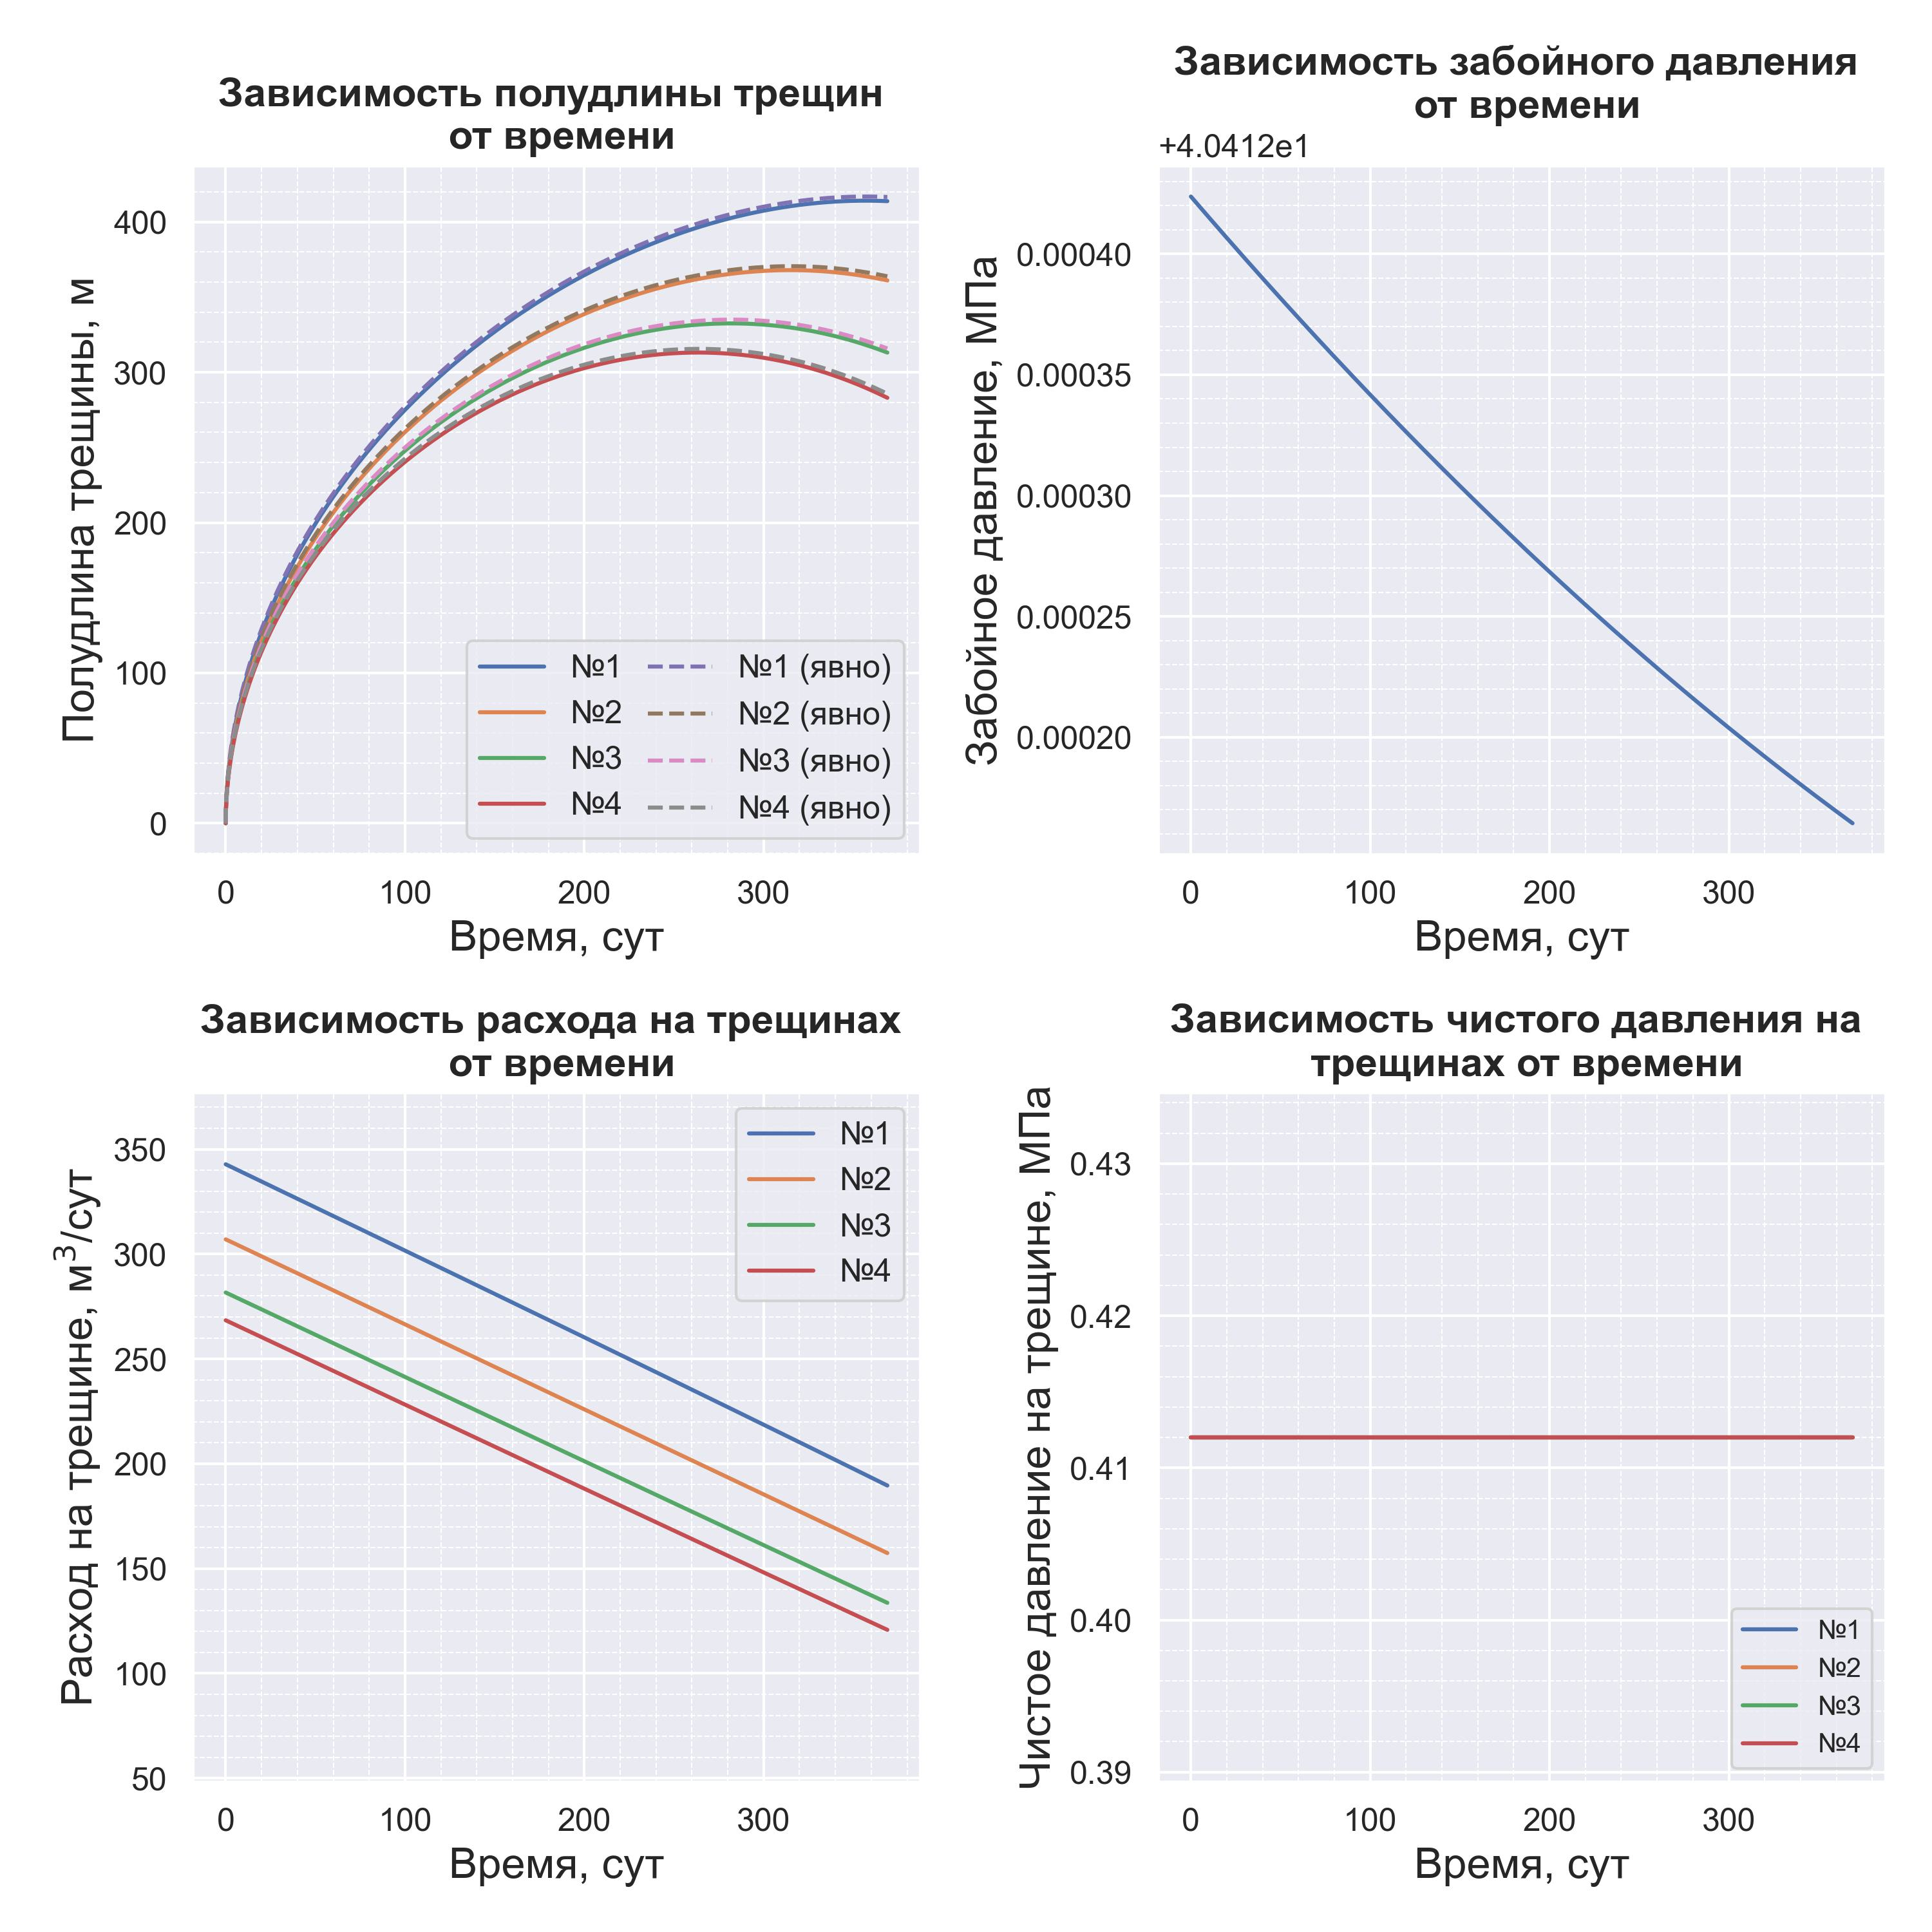
\includegraphics[width=\linewidth]{images/myimage6.jpg}
\caption{Результаты моделирования перераспределения потоков и роста трещин автоГРП в случае двумерных радиальных утечек жидкости из трещины в пласт и линейном уменьшении расхода жидкости на забое скважины}
\label{fig:myimage6}
\end{figure}

Также проведено моделирование роста трещин при изменении качества перфораций на одной из трещин.
Результаты представлены на рис. \ref{fig:myimage7} и рис. \ref{fig:myimage8}.
Ухудшение качества перфораций задавалось уменьшением диаметра перфораций на 2-ой трещине по следующей формуле:
\beq
d_{p,2}(t)=0.02\text{ м}-0.015\text{ м}\cdot\left(\frac{t}{365\text{ сут}}\right)
\eeq

\begin{figure}[H] 
\center
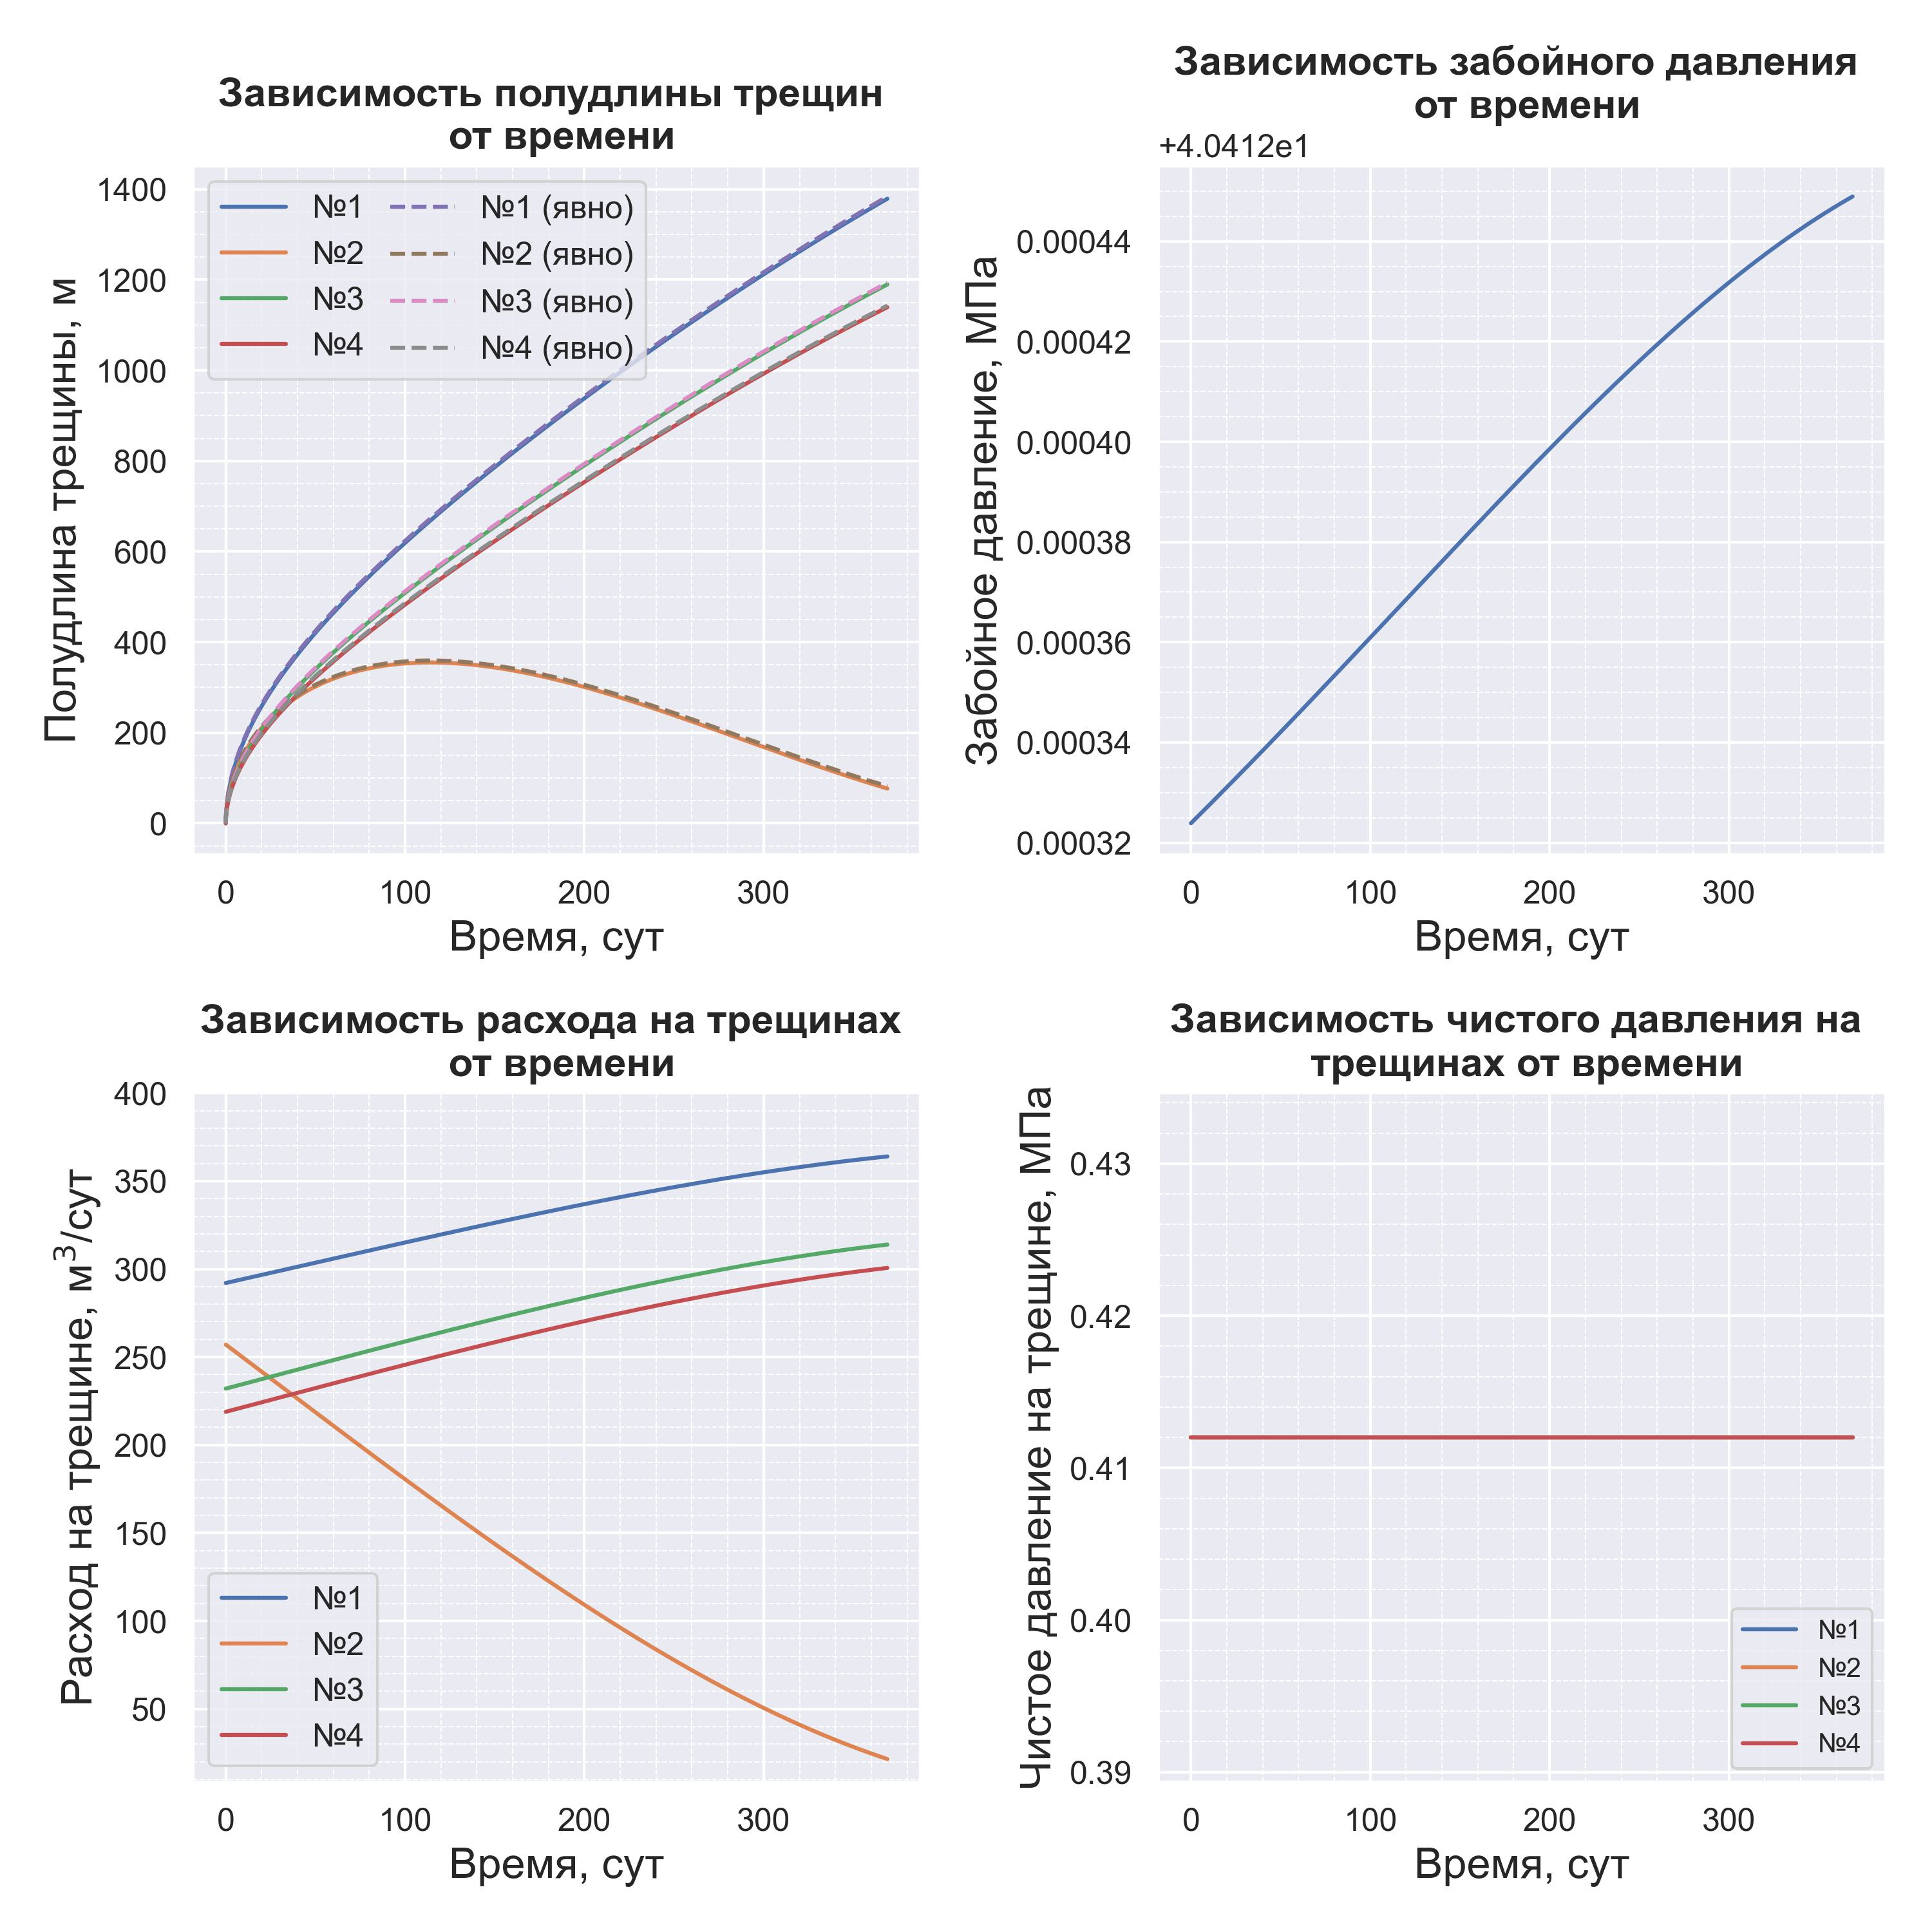
\includegraphics[width=\linewidth]{images/myimage7.jpg}
\caption{Результаты моделирования перераспределения потоков и роста трещин автоГРП при уменьшении диаметра перфораций на второй трещине (от 0.02 м до 0.005 м) -- режим утечек Картера}
\label{fig:myimage7}
\end{figure}

Видим, что ухудшение качества перфораций (уменьшение диаметра перфораций) на трещине приводит к её постепенному закрытию и одновременному сильному росту соседних трещин.

\begin{figure}[H] 
\center
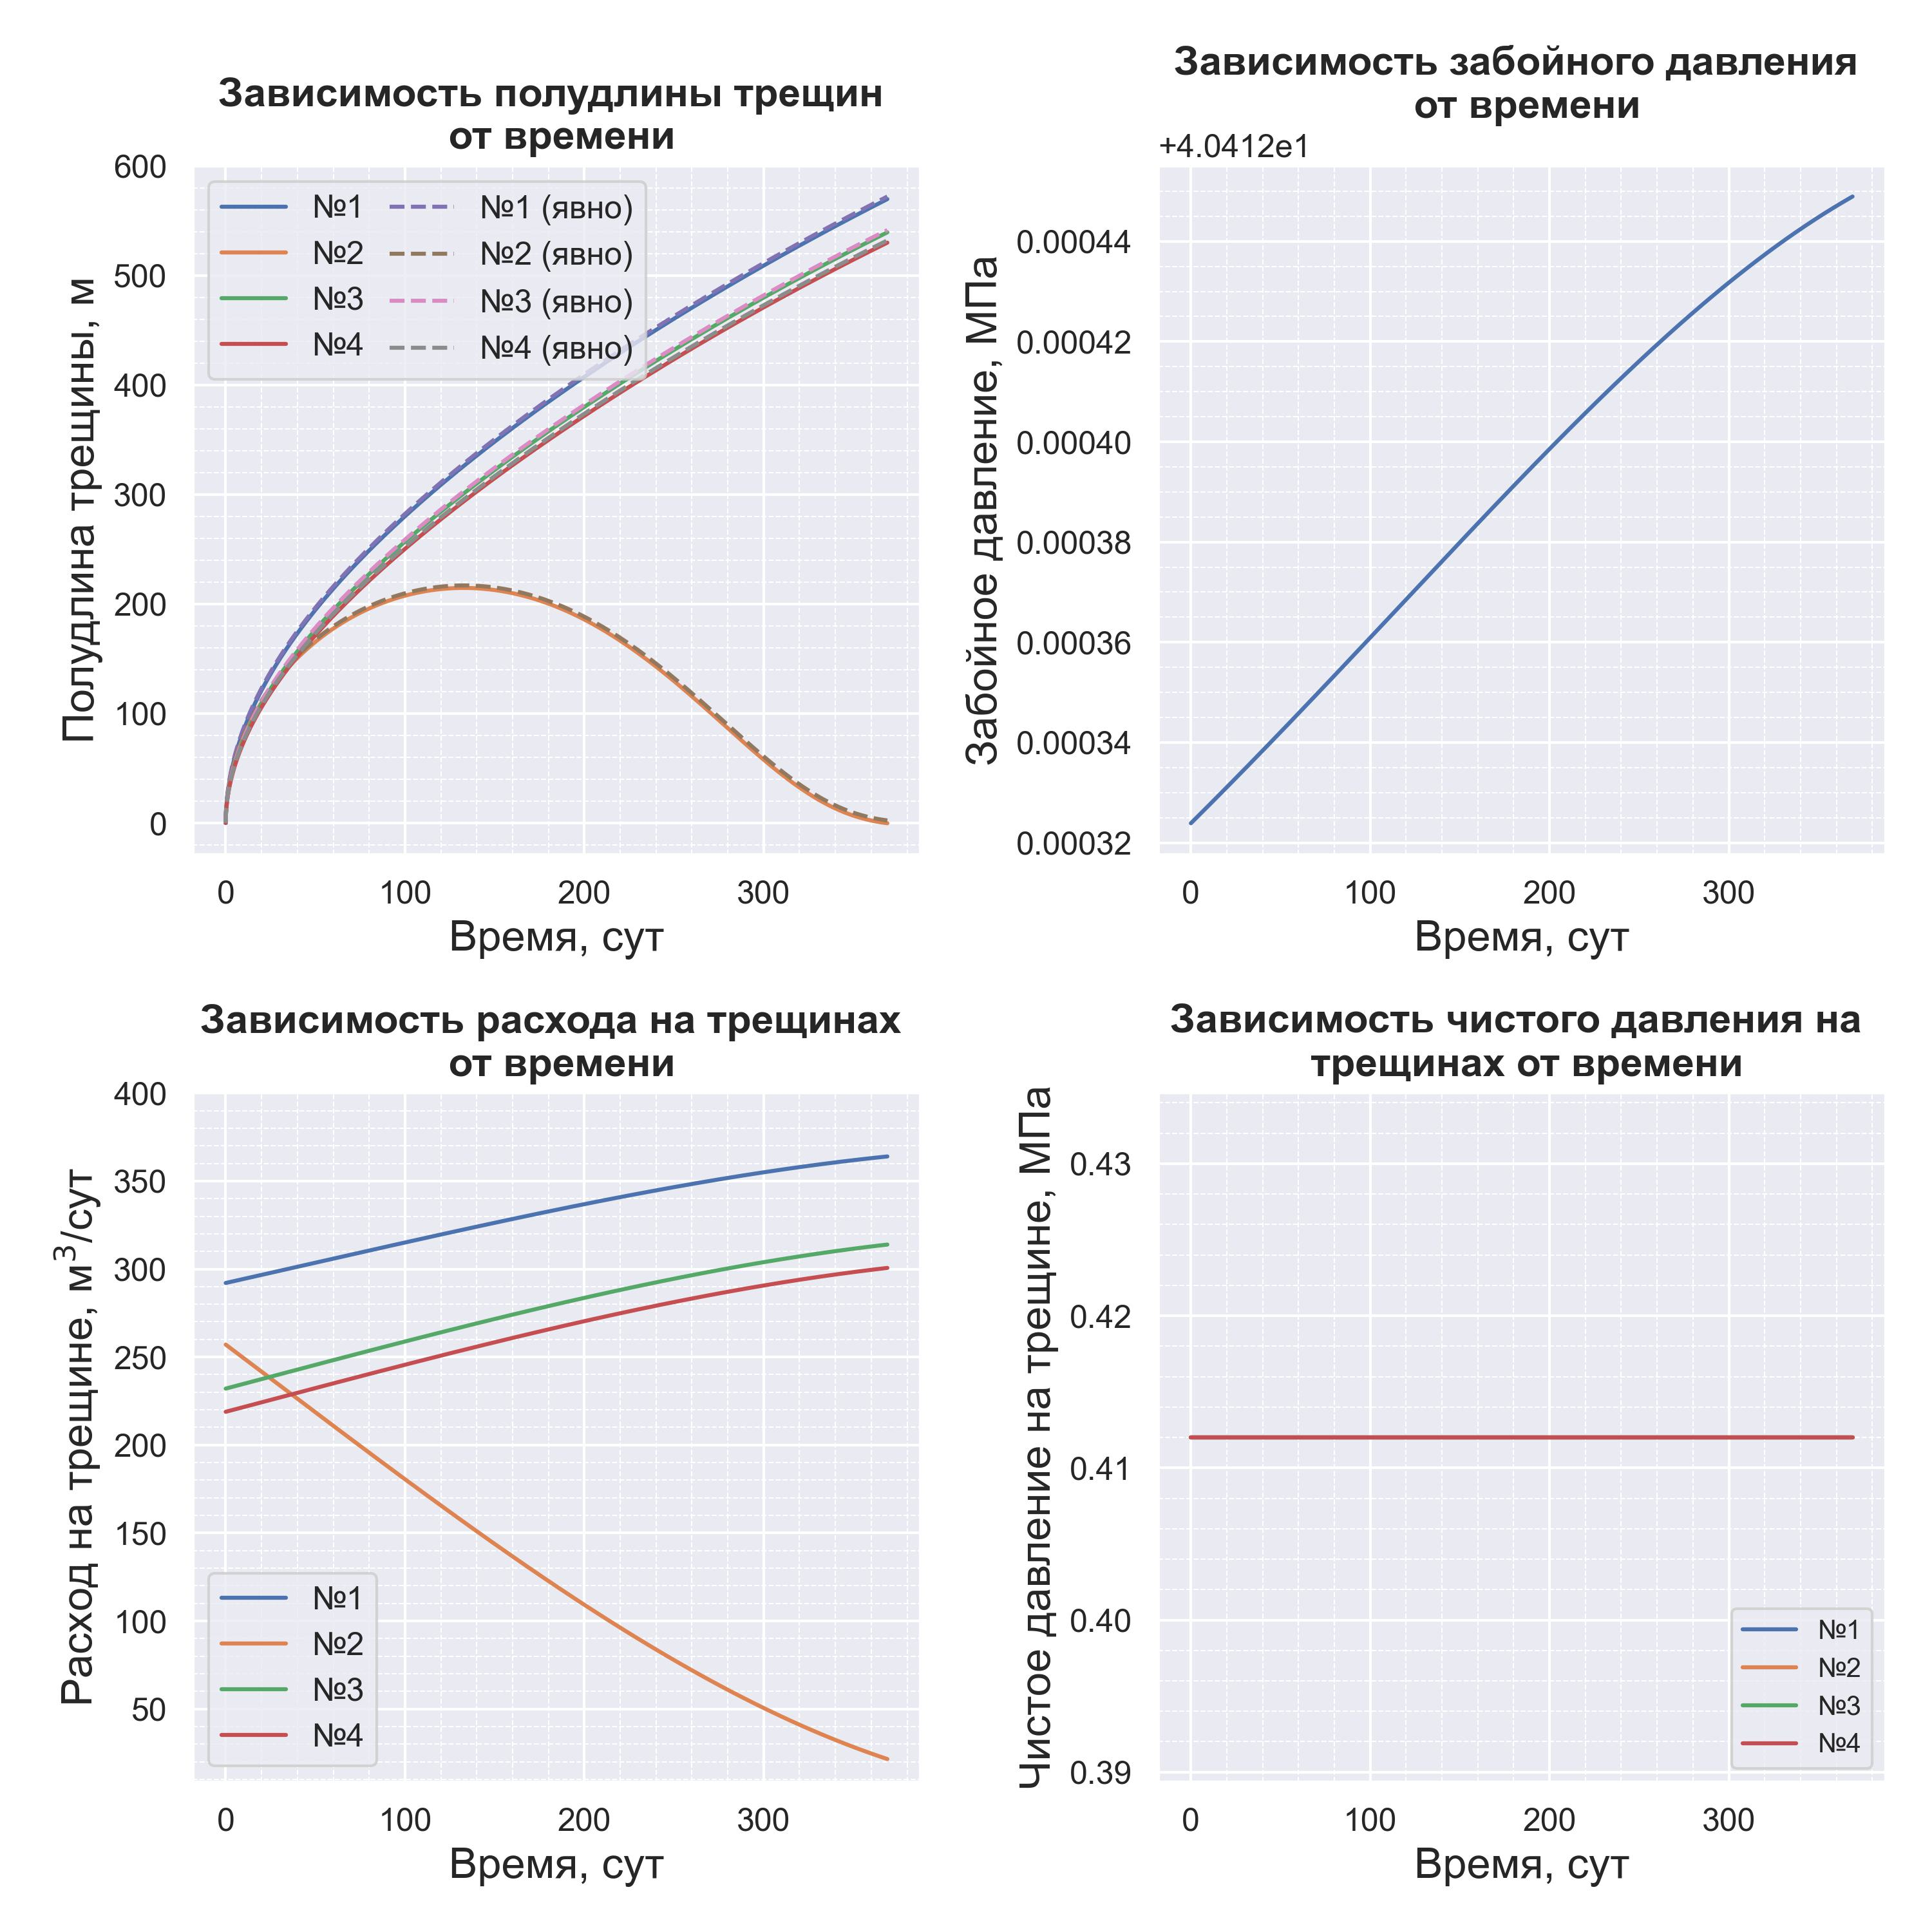
\includegraphics[width=\linewidth]{images/myimage8.jpg}
\caption{Результаты моделирования перераспределения потоков и роста трещин автоГРП при уменьшении диаметра перфораций на второй трещине (от 0.02 м до 0.005 м) -- двумерный радиальный режим утечек жидкости из трещины в пласт}
\label{fig:myimage8}
\end{figure}

При ухудшении качества перфораций на второй, третьей и четвёртой трещинах наблюдается интересная картина (см. рис. \ref{fig:myimage9} и рис. \ref{fig:myimage10}) стремительного роста первой трещины, на которой качество перфораций не изменяется.
Особенно сильно этот эффект заметен в случае одномерных утечек Картера.

Диаметр перфораций на второй, третьей и четвёртой трещинах изменялся по следующим формулам:
\beq
d_{p,2}(t)=0.02\text{ м}-0.015\text{ м}\cdot\left(\frac{t}{365\text{ сут}}\right)
\eeq
\beq
d_{p,3}(t)=0.02\text{ м}-0.010\text{ м}\cdot\left(\frac{t}{365\text{ сут}}\right)
\eeq
\beq
d_{p,4}(t)=0.02\text{ м}-0.005\text{ м}\cdot\left(\frac{t}{365\text{ сут}}\right)
\eeq

\begin{figure}[H] 
\center
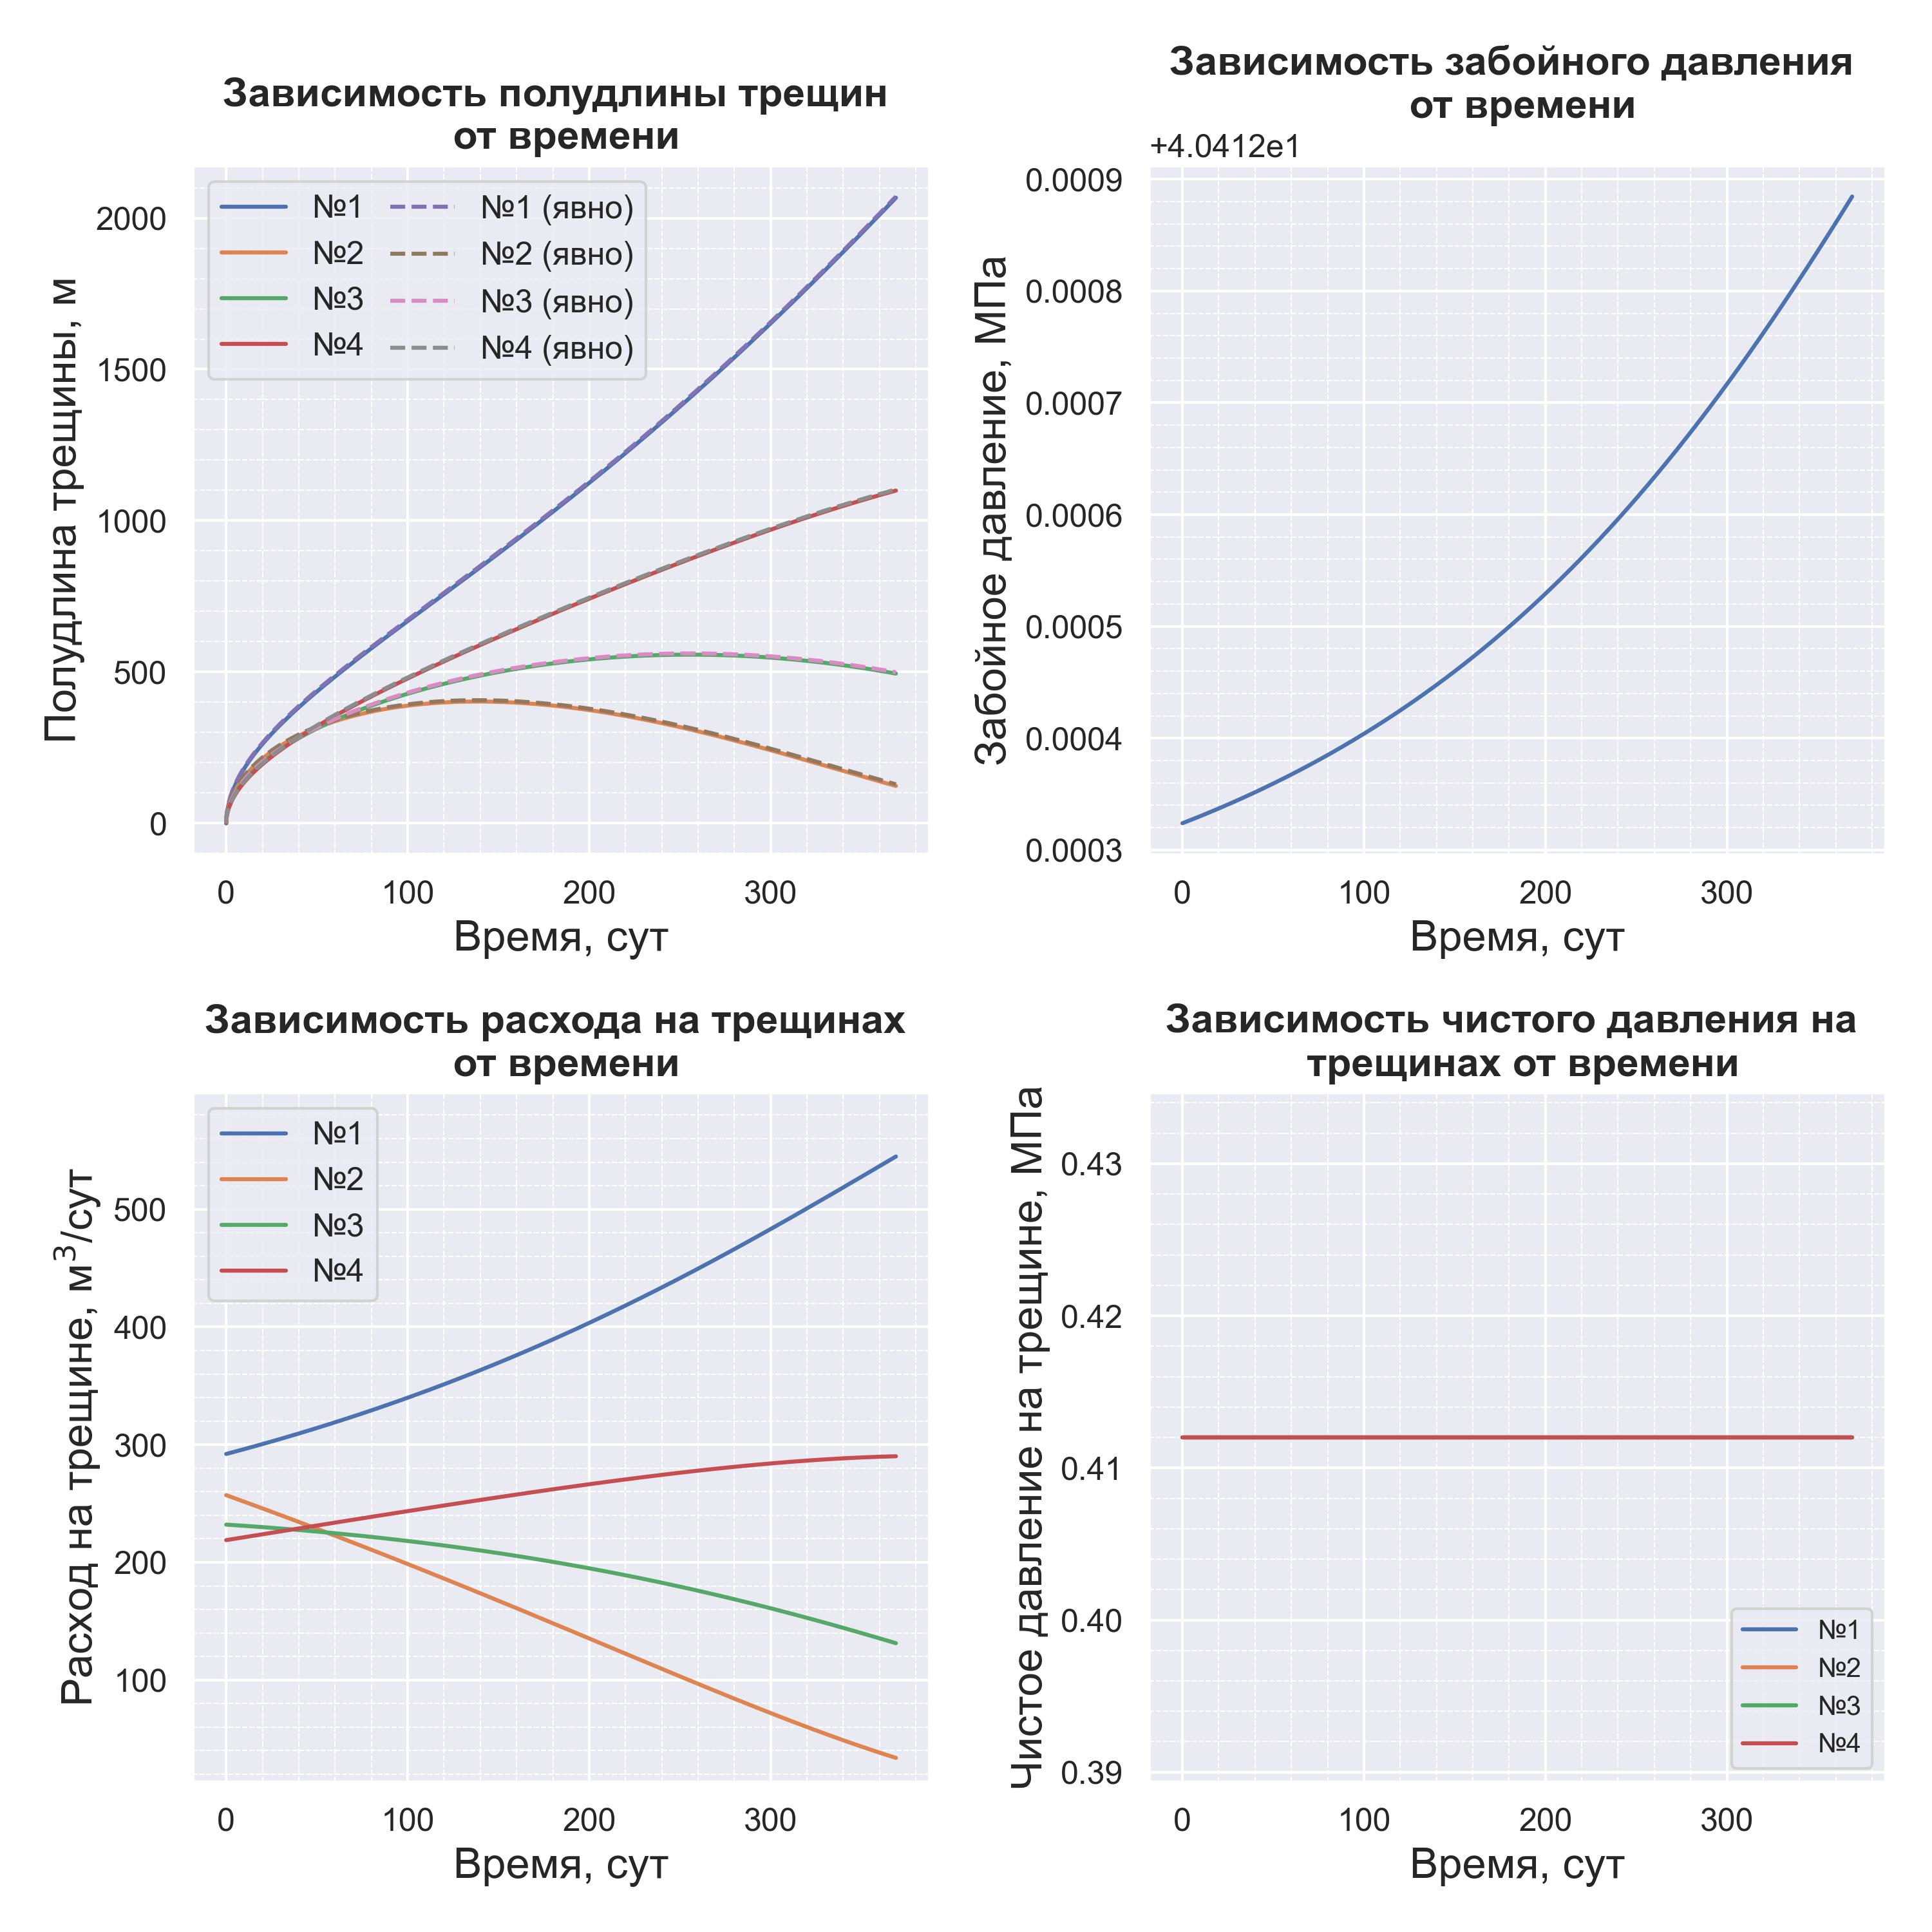
\includegraphics[width=\linewidth]{images/myimage9.jpg}
\caption{Результаты моделирования перераспределения потоков и роста трещин автоГРП при уменьшении диаметра перфораций на второй, третьей и четвёртой трещинах -- режим утечек Картера}
\label{fig:myimage9}
\end{figure}


\begin{figure}[H] 
\center
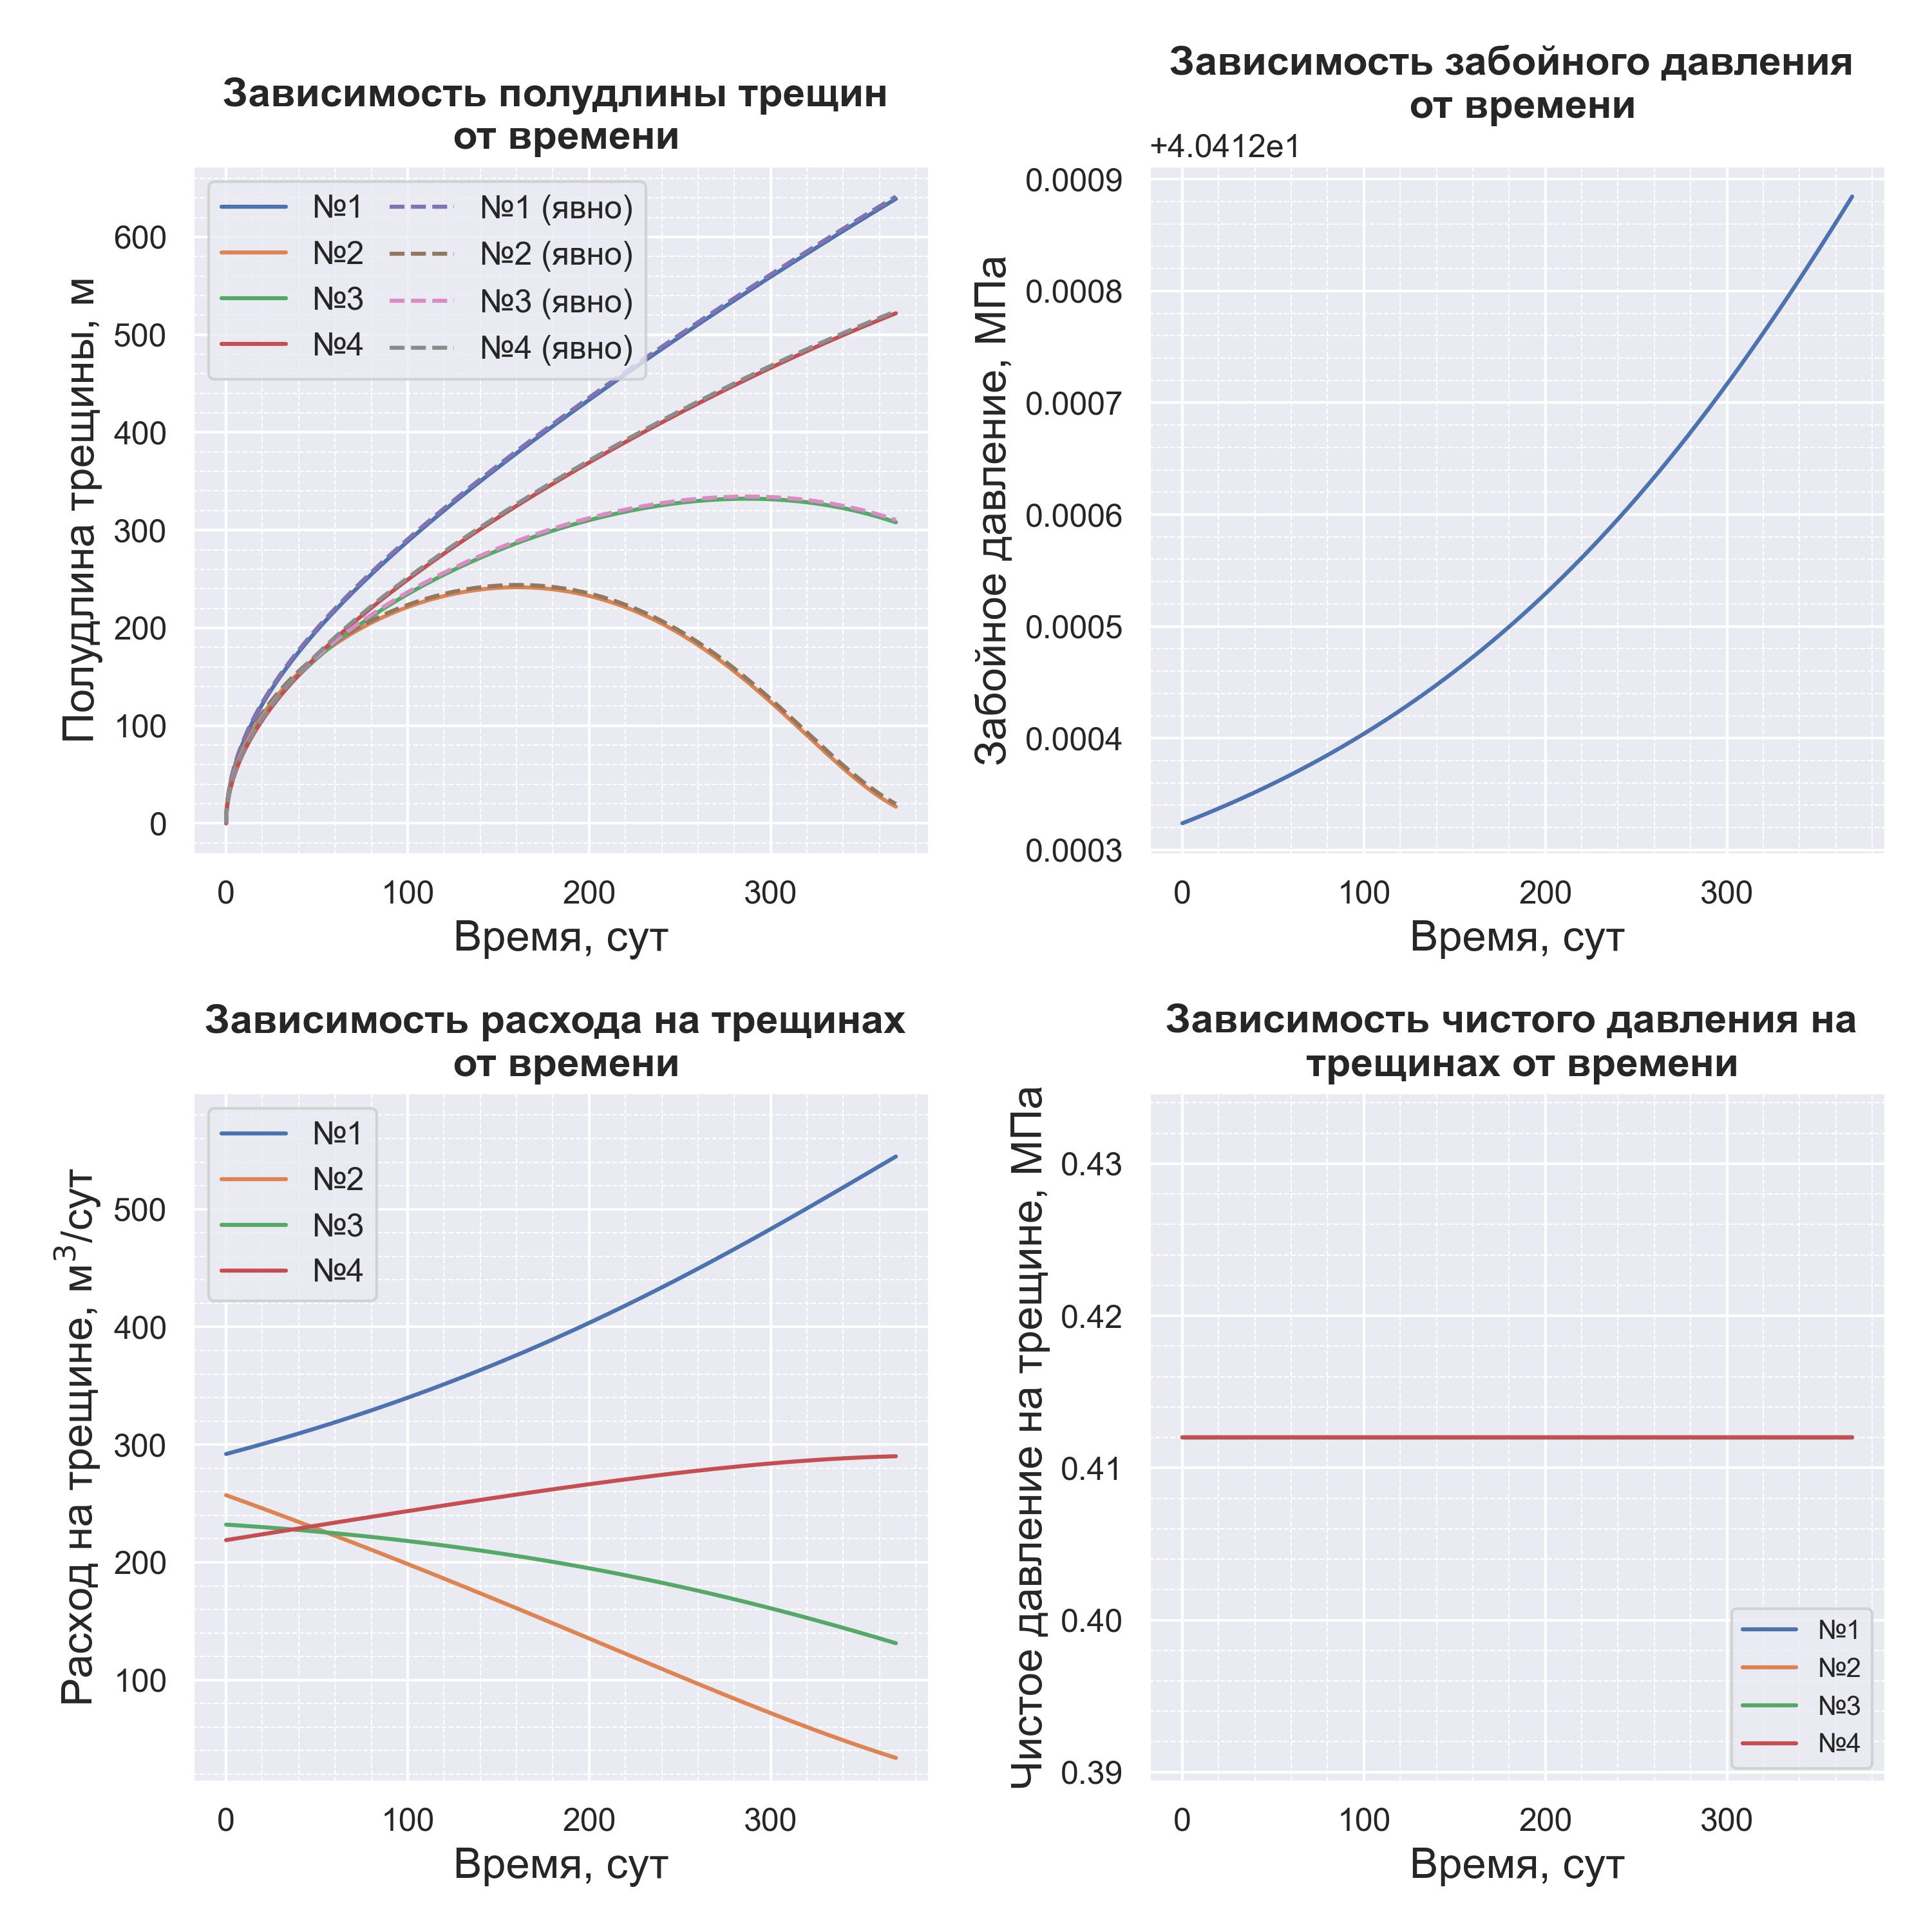
\includegraphics[width=\linewidth]{images/myimage10.jpg}
\caption{Результаты моделирования перераспределения потоков и роста трещин автоГРП при уменьшении диаметра перфораций на второй, третьей и четвёртой трещинах -- двумерный радиальный режим утечек жидкости из трещины в пласт}
\label{fig:myimage10}
\end{figure}

Далее проведён эксперимент при уменьшении горизонтальных напряжений в пласте со временем (за счёт термоупругого воздействия -- например, в пласт закачивается холодная вода).
Результаты представлены на рис. \ref{fig:myimage11} и \ref{fig:myimage12}.
Минимальное горизонтальное напряжение в пласте в этом эксперименте изменялось по формуле:
\beq
\sigma_{\text{min}}(t)=40\text{ МПа}-5\text{ МПа}\cdot\left(\frac{t}{365\text{ сут}}\right)
\eeq

\begin{figure}[H] 
\center
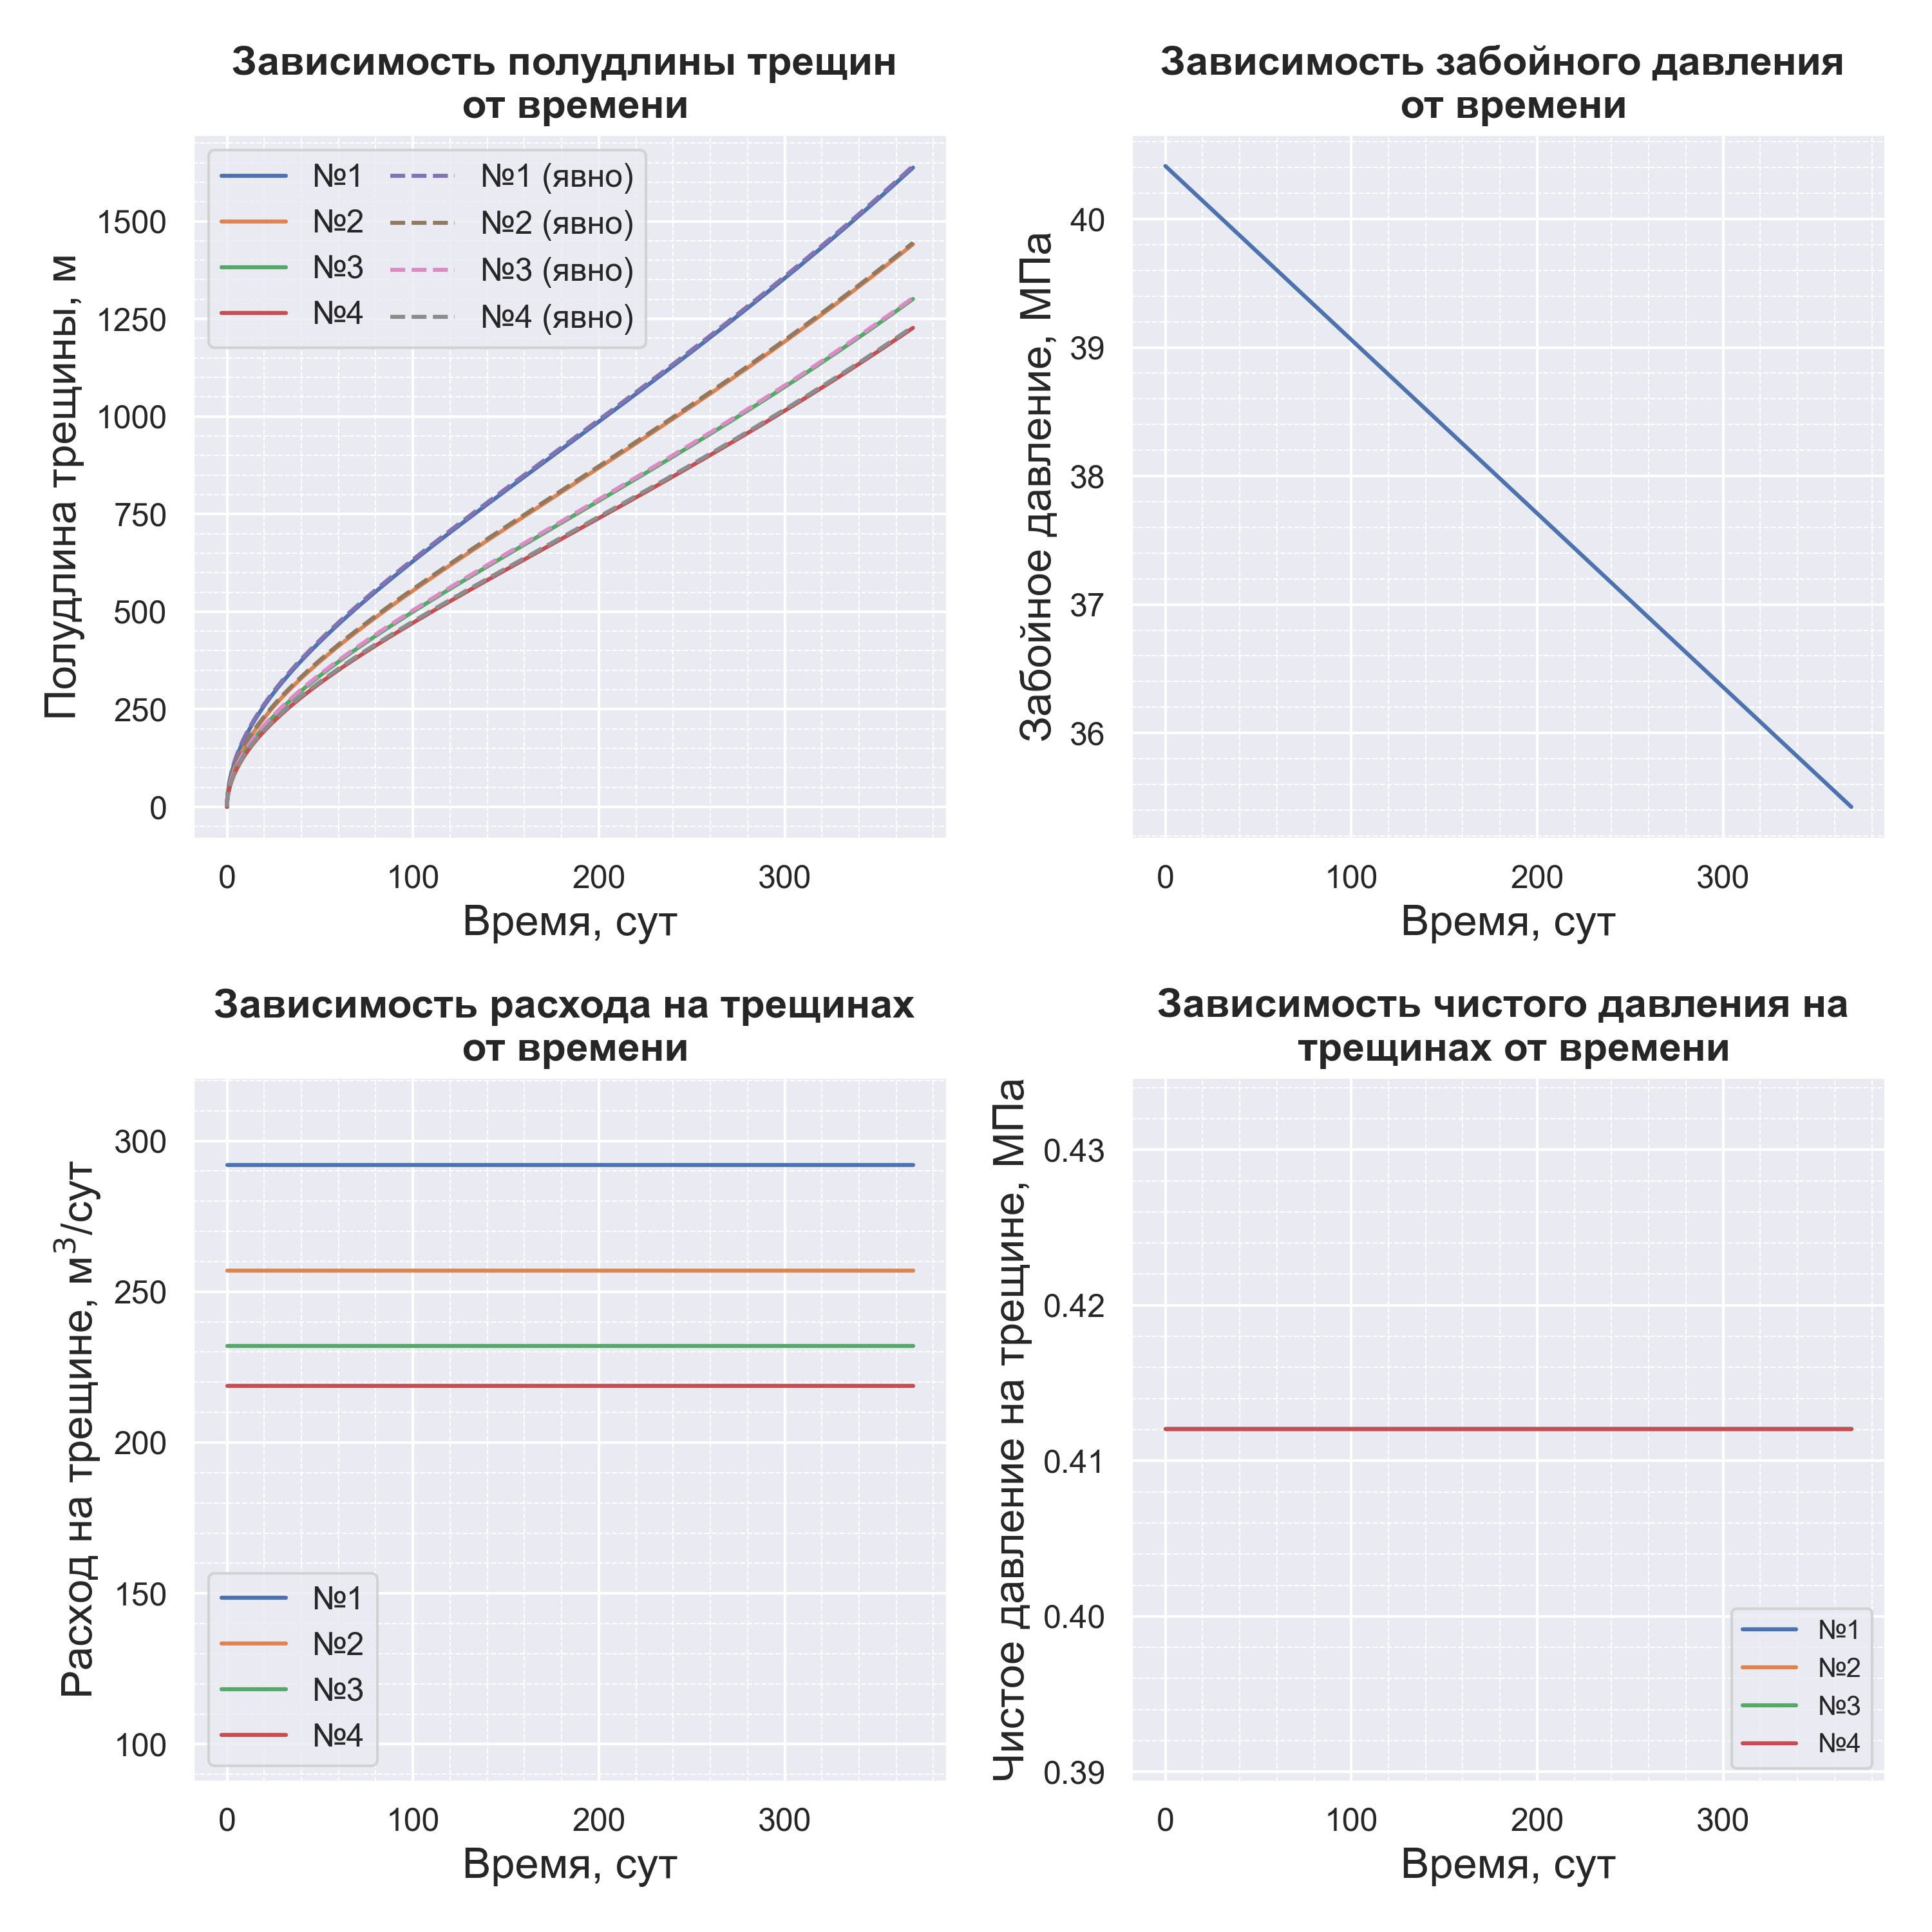
\includegraphics[width=\linewidth]{images/myimage11.jpg}
\caption{Результаты моделирования перераспределения потоков и роста трещин автоГРП при термоупругом воздействии (уменьшении горизонтальных напряжений в пласте) -- режим утечек Картера}
\label{fig:myimage11}
\end{figure}

Из рис. \ref{fig:myimage11} и рис. \ref{fig:myimage12} видим, что термоупругое уменьшение горизонтальных напряжений в пласте  приводит к более длинным трещинам (по сравнению с базовым сценарием рис. \ref{fig:myimage1} и \ref{fig:myimage2}), что согласуется с результатами работы \cite{perkins_gonzalez}.

\begin{figure}[H] 
\center
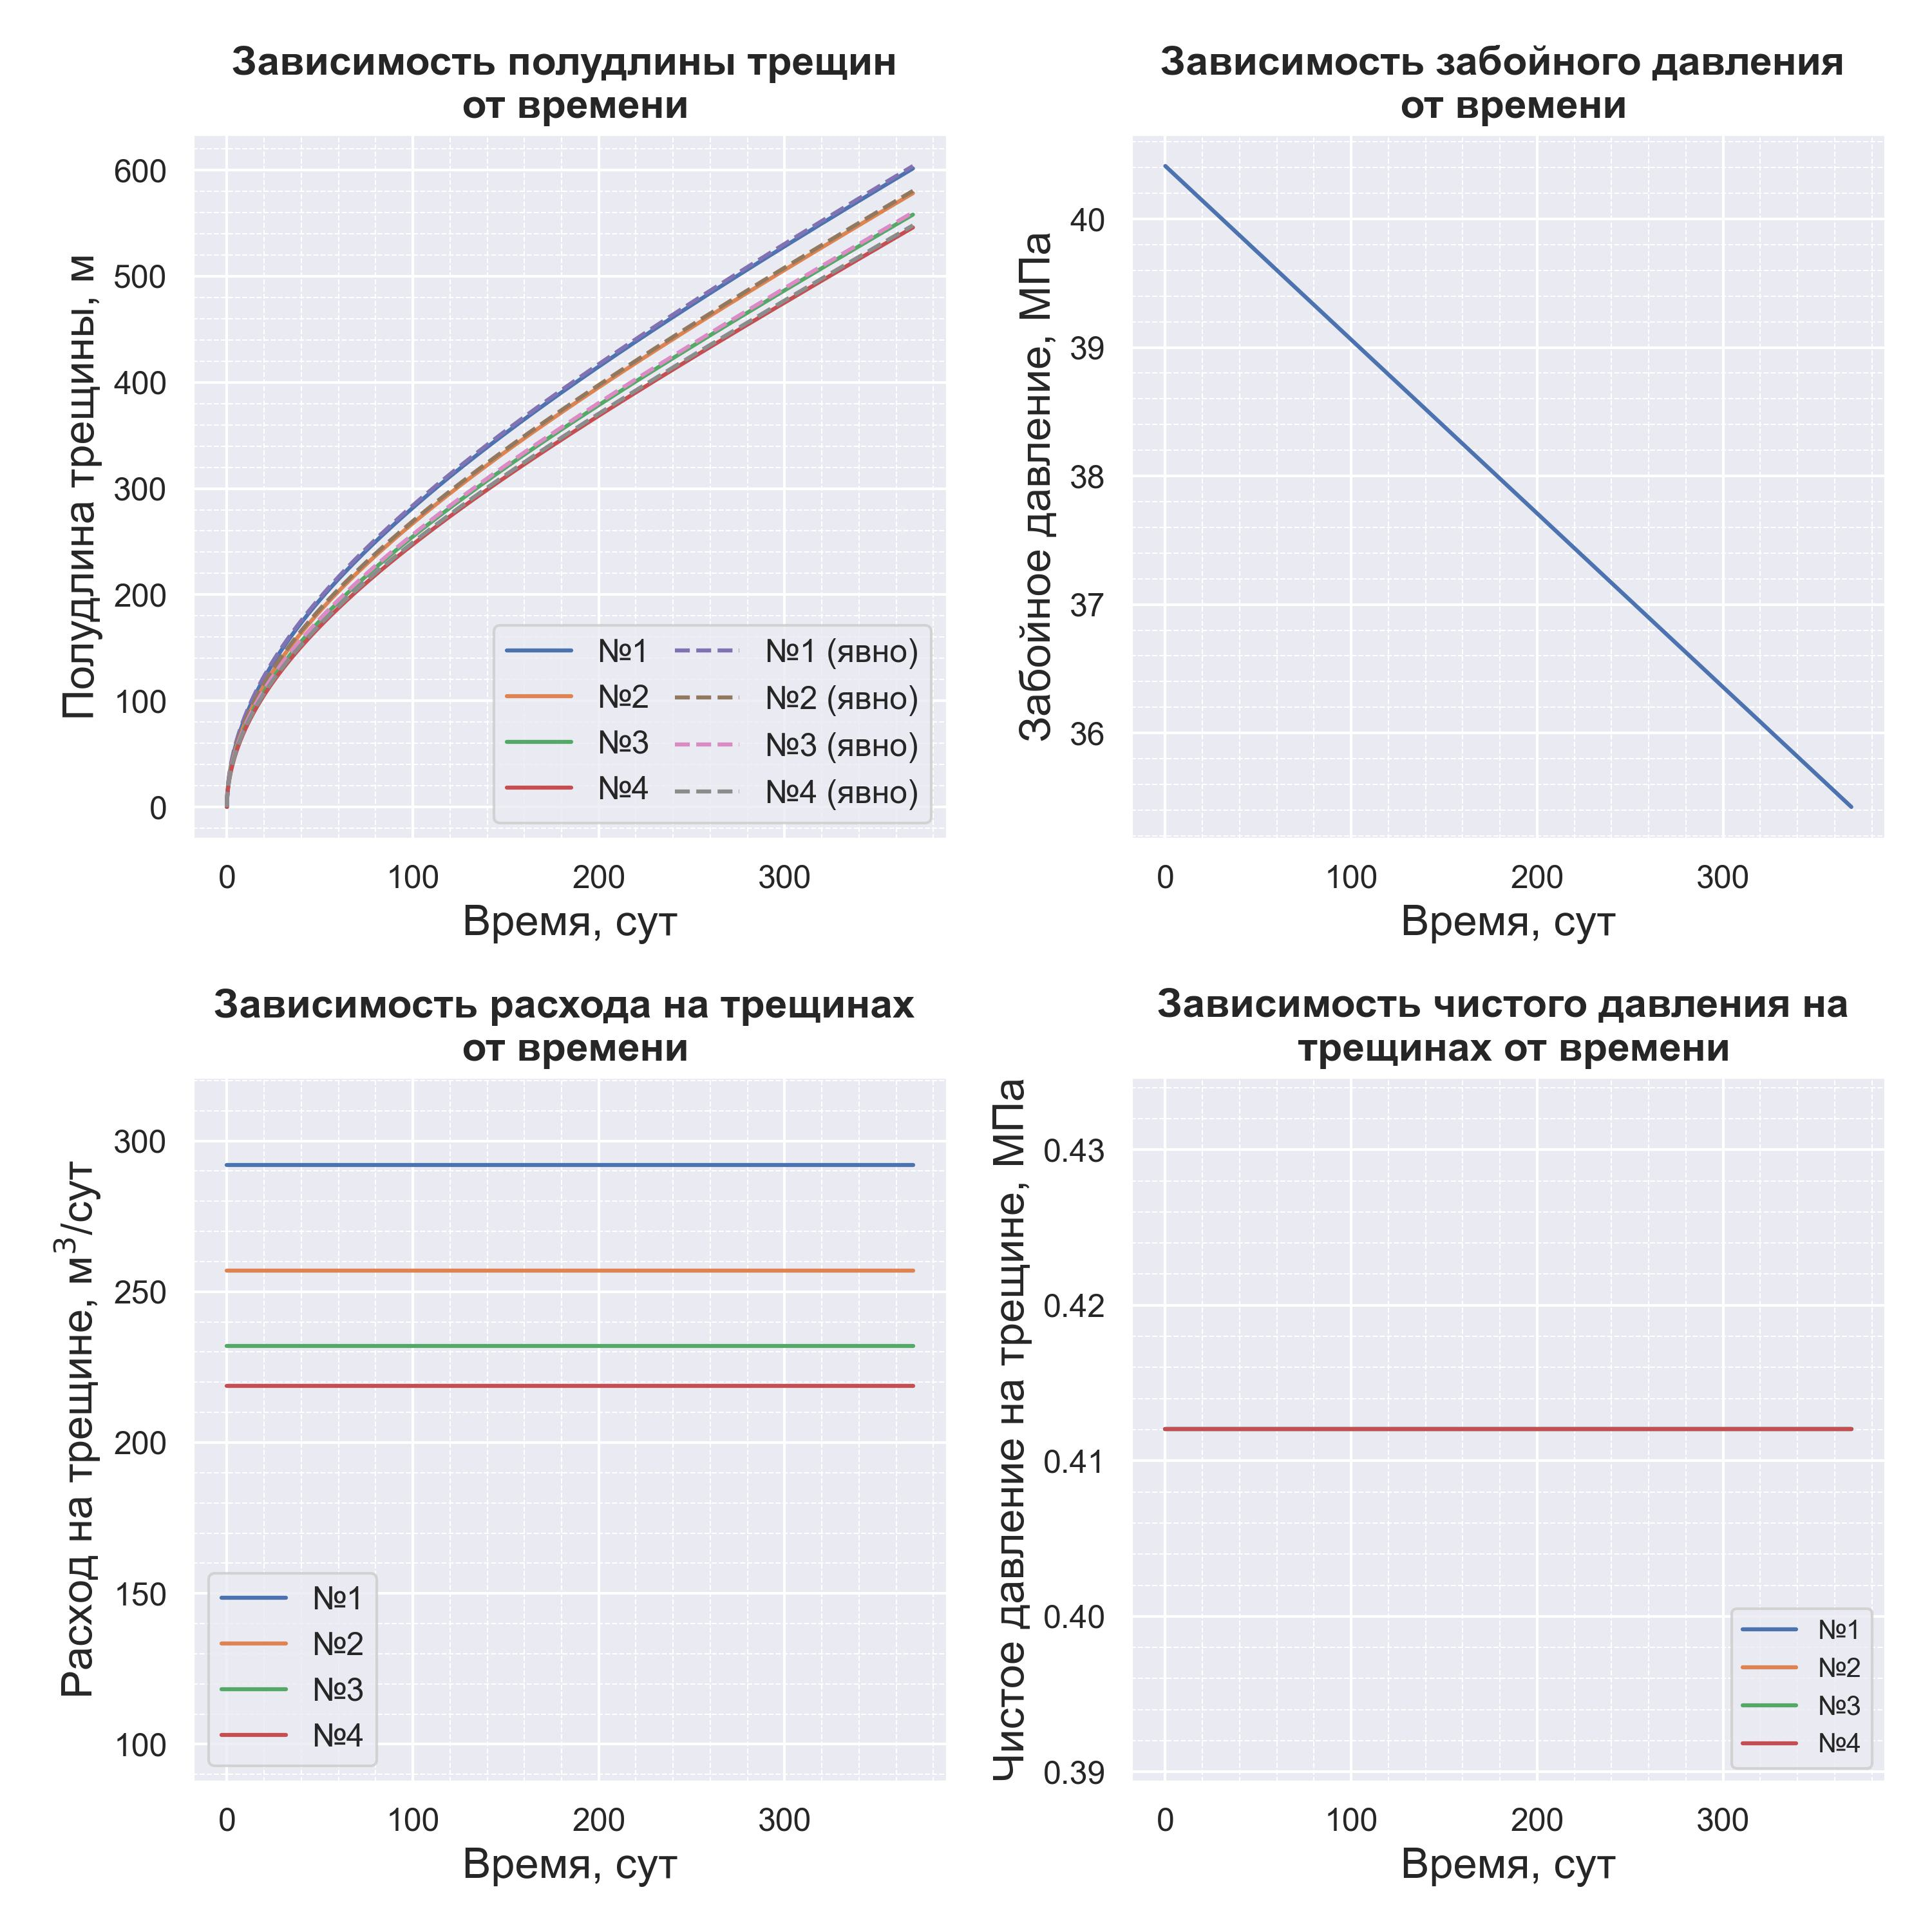
\includegraphics[width=\linewidth]{images/myimage12.jpg}
\caption{Результаты моделирования перераспределения потоков и роста трещин автоГРП при термоупругом воздействии (уменьшении горизонтальных напряжений в пласте) -- двумерный радиальный режим утечек жидкости из трещины в пласт}
\label{fig:myimage12}
\end{figure}

Дополнительно для проверки работоспособности построенного алгоритма проведён эксперимент при одновременном росте шести трещин.
При этом на третьей трещине со временем уменьшается диаметр перфораций.
Результаты представлены на рис. \ref{fig:myimage13}.

\begin{figure}[H] 
\center
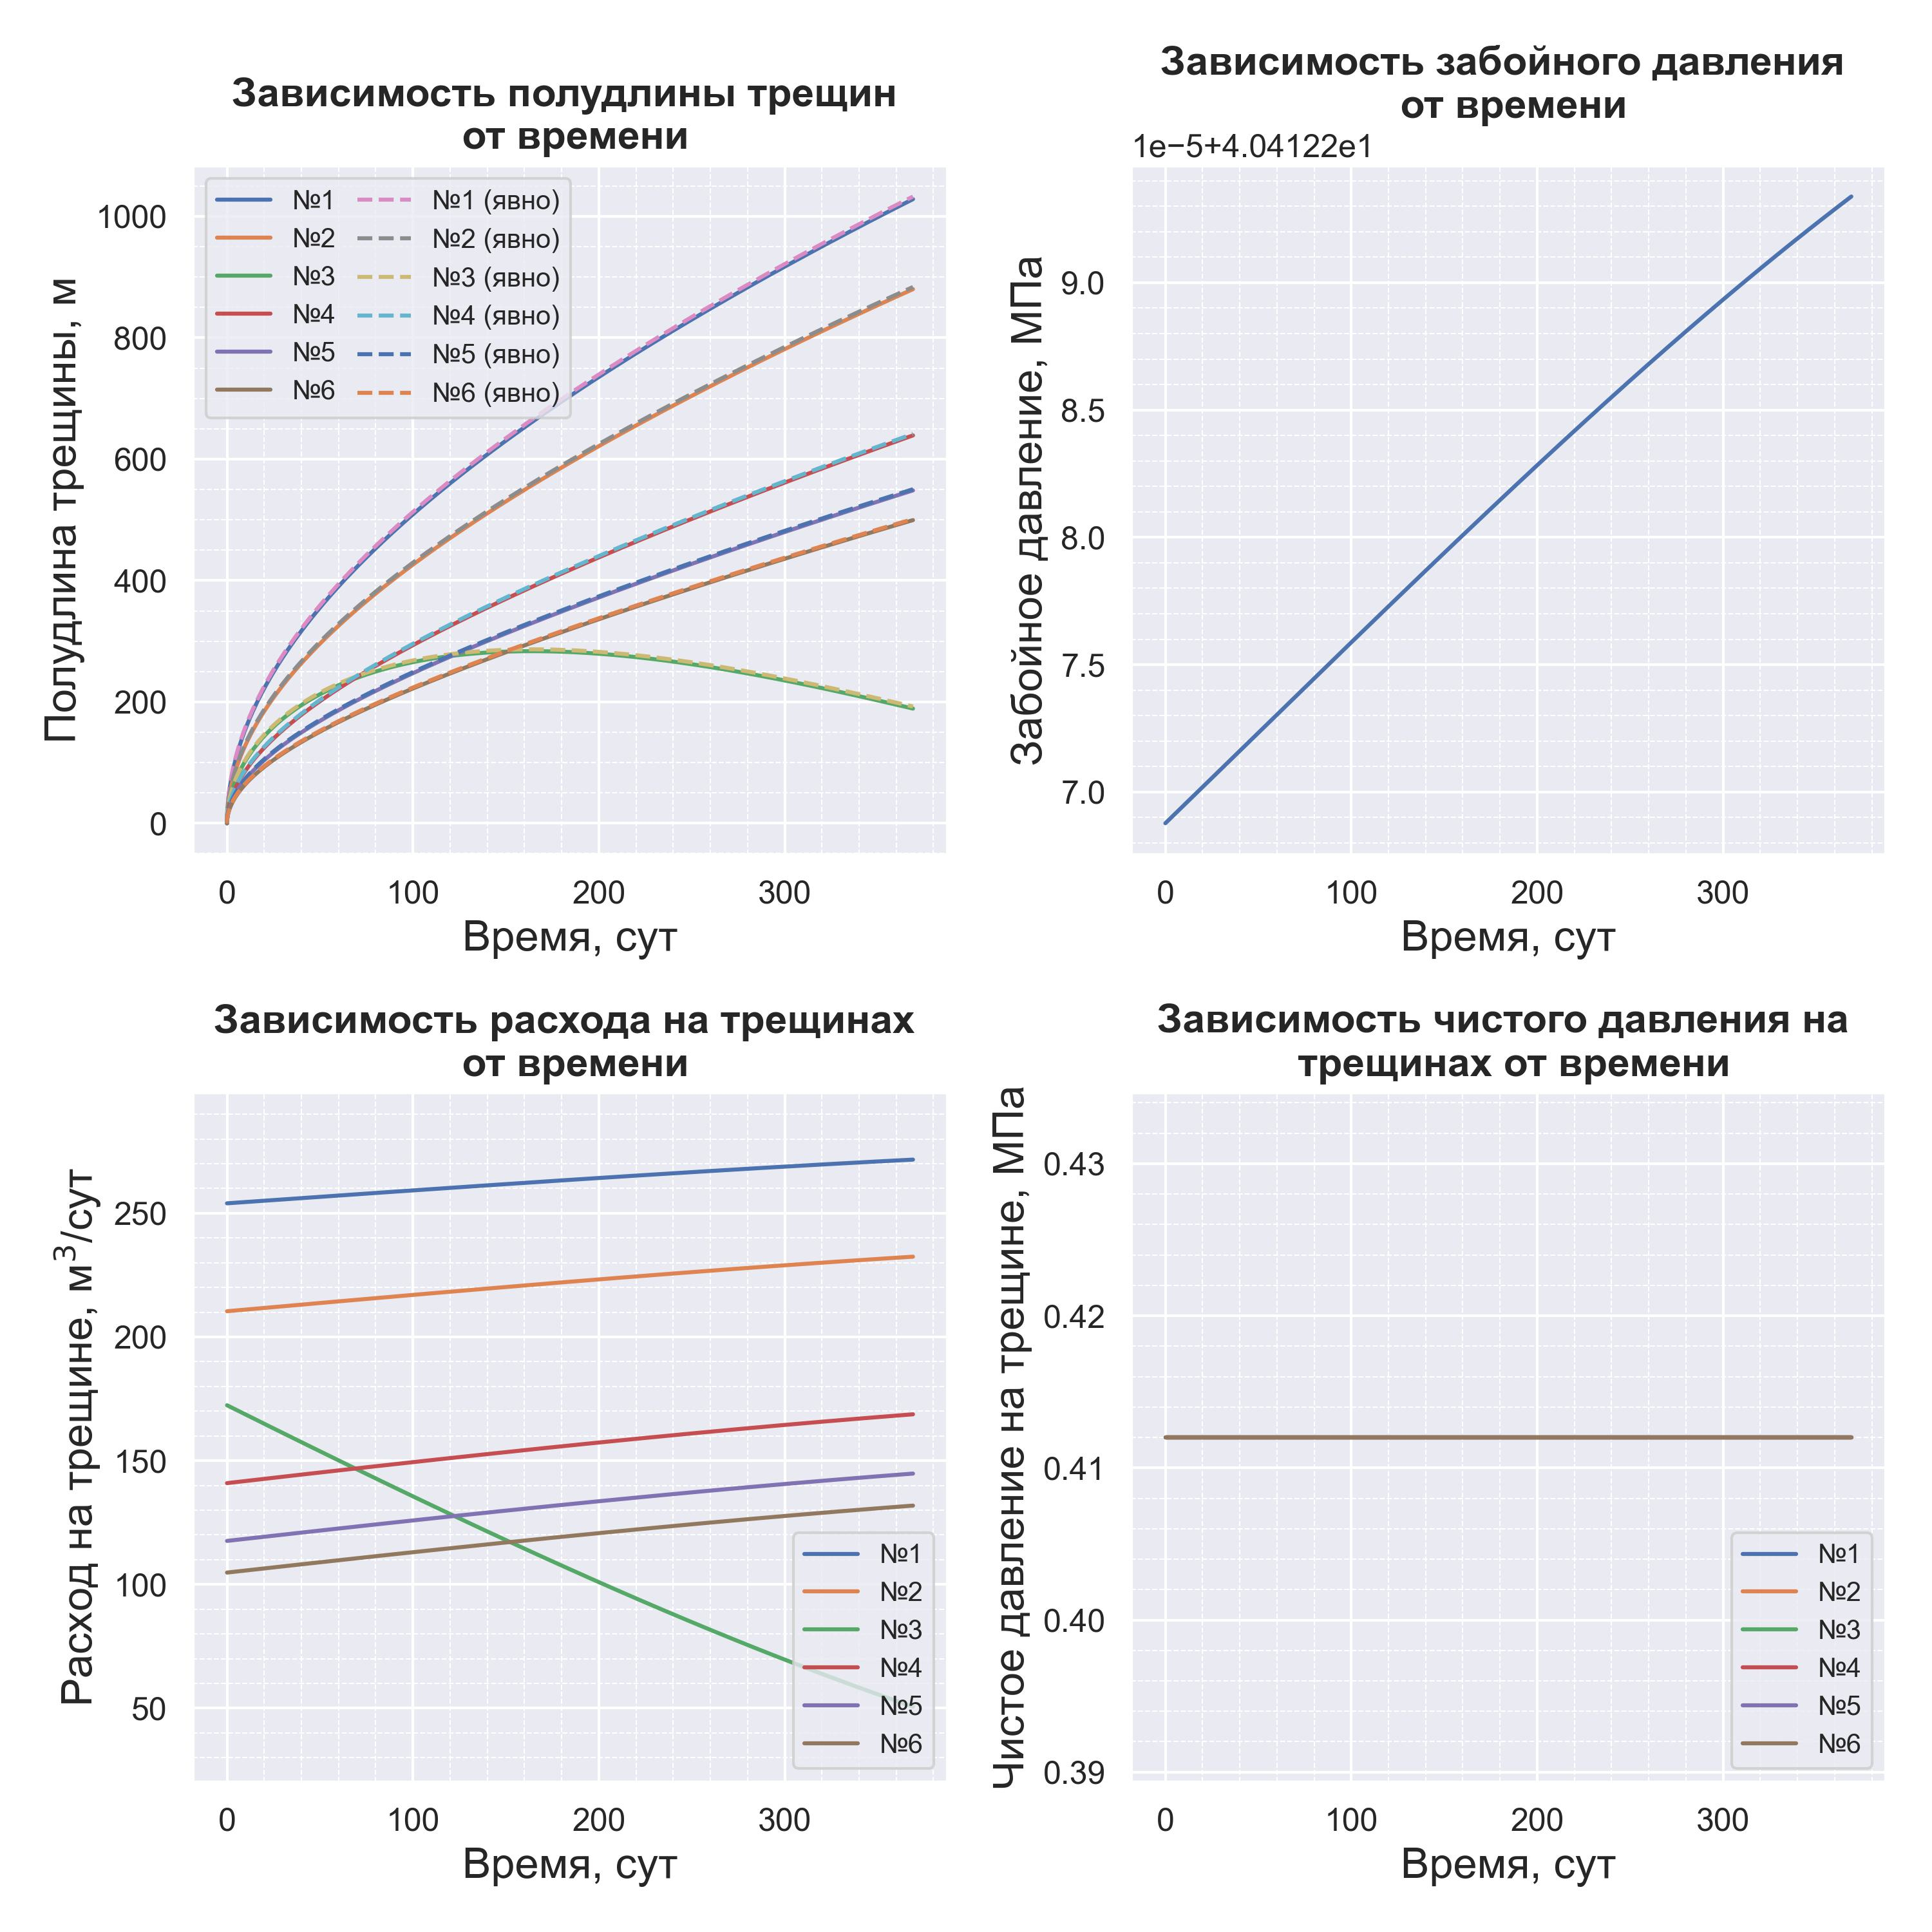
\includegraphics[width=\linewidth]{images/myimage13.jpg}
\caption{Результаты моделирования перераспределения потоков и роста трещин автоГРП при одновременном росте шести трещин и уменьшении диаметра перфораций на трещине №3 -- режим утечек Картера}
\label{fig:myimage13}
\end{figure}

Видим, что уменьшение диаметра перфораций на одной из трещин приводит к уменьшению длины этой трещины и одновременному более интенсивному росту соседних трещин.

%
%\begin{figure}[H]
%	\adjustbox{minipage=1.3em,valign=t}{\subcaption{}\label{fig:p_0(q_0)}}%
%	\begin{subfigure}[t]{\dimexpr.5\linewidth-1.3em\relax}
%		\centering
%		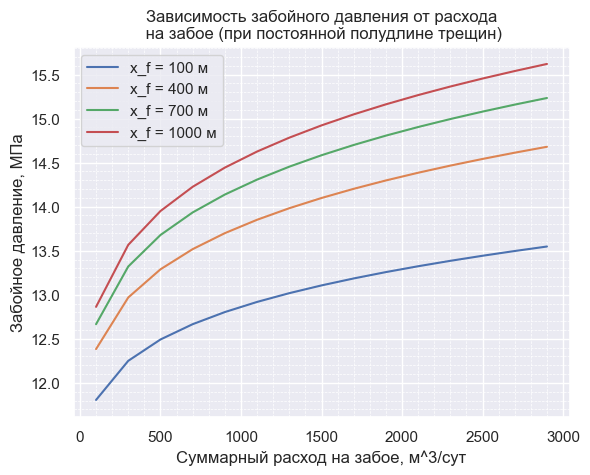
\includegraphics[width=.95\linewidth,valign=t]{images/p_0(q_0).png}
%	\end{subfigure}
%\hfill %выровнять по ширине
%	\adjustbox{minipage=1.3em,valign=t}{\subcaption{}\label{fig:p_0(x_f)}}%
%	\begin{subfigure}[t]{\dimexpr.5\linewidth-1.3em\relax}
%		\centering
%		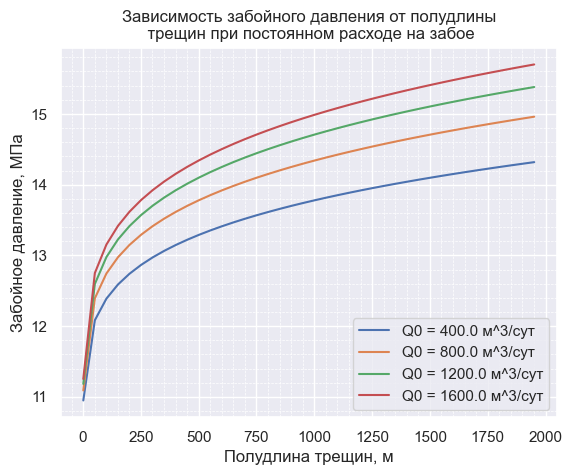
\includegraphics[width=.95\linewidth,valign=t]{images/p_0(x_f).png}
%	\end{subfigure}
%\captionsetup{justification=centering} %центрировать
%\caption{Зависимости забойного давления от основных параметров задачи: {\itshape a} --- от суммарного расхода на забое; {\itshape b} --- от полудлины трещин} 
%\label{fig:results1}
%\end{figure}

%Результаты моделирования представлены на рис. \ref{fig:results2}.
 
%\begin{figure}[H] 
%\center
%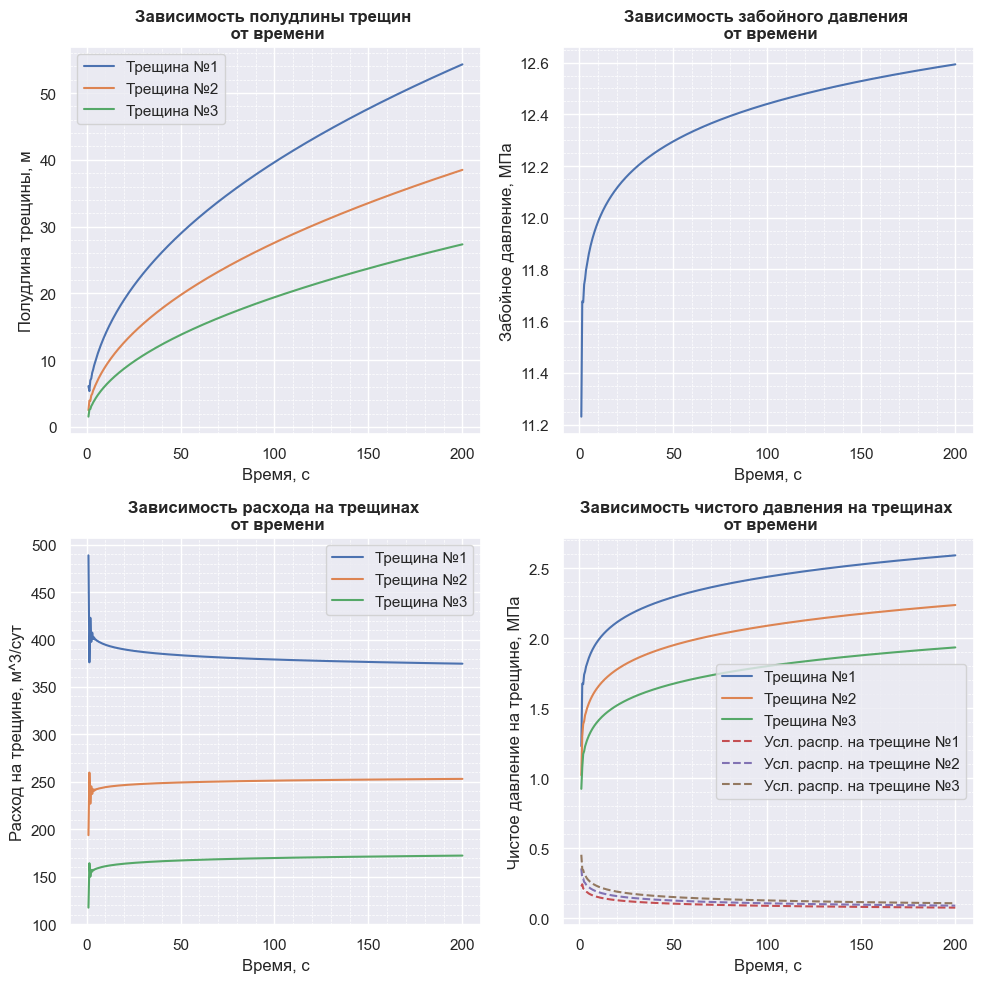
\includegraphics[width=.85\linewidth]{images/Kirchhoff+Koning.png}
%\caption{Результаты решения поставленной задачи} 
%\label{fig:results2}  
%\end{figure}

%В проведённом численном эксперименте трещины отличаются друг от друга количеством и диаметром перфораций.\newline
%У трещины 1: количество перфораций 32, диаметр перфораций 0.02 м.\newline
%У трещины 2: количество перфораций 2, диаметр перфораций 0.01 м.\newline
%У трещины 3: количество перфораций 1, диаметр перфораций 0.01 м.
%\\

%Код решения представлен по ссылке: \url{https://github.com/mualal/hydrofracturing/blob/master/notebooks/02_fractures_growth_with_Koning.ipynb}

%Из графиков на рис. \ref{fig:results2} видим, что большую часть потока забирает на себя трещина с лучшими перфорациями.
%Эта же трещина лидирует по скорости роста.

%Также видим, что при росте трещин требуется всё большее забойное давление для того, чтобы поддерживать этот рост.

%При выбранных входных параметрах построенной модели чистое давление в каждой из трещин существенно превышает давления критерия распространения, следовательно, при достаточно высоком забойном давлении все трещины будут расти одновременно.
